\documentclass[a4paper,10pt]{article}
\usepackage{a4wide}
\usepackage{amsmath}
\usepackage{amssymb}
%\usepackage{empheq}
\usepackage[english]{babel}
\usepackage{graphicx}
\usepackage{enumerate}
\usepackage{subcaption,array}
\usepackage{multicol}
\usepackage{csvsimple}
%\usepackage{mathtools}
\usepackage{latexsym}
\usepackage{fullpage}
\usepackage{verbatim}
\usepackage{algorithm}
\usepackage{algpseudocode}
\usepackage{float}
\usepackage{bbm}
\usepackage[section]{placeins} % Prevent floats from passing beyond \FloatBarrier; keep floats within their sections
\usepackage{appendix}
\usepackage{import} %tex bestanden importeren deze moeten alleen tekst bevatten geen \begin{document} etc.
\usepackage{listings}
\usepackage{eurosym}
\usepackage[utf8]{inputenx}
\usepackage{program}
\usepackage{bookmark}

\newcommand{\desda}{\Leftrightarrow}
\newcommand{\rr}{\mathbb{R}}
\newcommand{\nn}{\mathbb{N}}
\newcommand{\zz}{\mathbb{Z}}
\newcommand{\qq}{\mathbb{Q}}
\newcommand{\rn}{\mathbb{R}^n}
\newcommand{\fdr}{f:D\rightarrow \rr}
\newcommand{\ul}{\underline}
\newcommand{\pp}{\mathbb{P}}
\newcommand{\ee}{\mathbb{E}}
\newcommand{\lnn}{\tilde{L}_n}
\newcommand{\convdis}{\overset{d}{\longrightarrow}}



\newcommand{\onaf}{\perp\!\!\!\perp}
\newcommand\red[1]{{\color{red}#1}} %kleurt text rood


\lstset{                         %settings voor code, zie ook http://en.wikibooks.org/wiki/LaTeX/Source_Code_Listings
breaklines=true,                 % sets automatic line breaking
commentstyle=\color{mygreen},    % comment style
%frame=single,                    % adds a frame around the code
keywordstyle=\color{blue},       % keyword style    \bfseries voor Bold
numberstyle=\tiny\color{black}, % the style that is used for the line-numbers
rulecolor=\color{black},         % if not set, the frame-color may be changed on line-breaks within not-black text
numbers=left,                    % where to put the line-numbers; possible values are (none, left, right)
}
\setlength\parindent{0pt}
\renewcommand\lstlistlistingname{Lijst van listings}
\usepackage{color}                  %Voor kleuren, o.a. in code
\usepackage{xcolor}                 %Voor kleuren, werkend krijgen  van box boven code
\definecolor{mygreen}{rgb}{0,0.6,0} %groene kleur voor comments in code
\usepackage{caption}
\DeclareCaptionFont{white}{\color{white}}
%\DeclareCaptionFormat{listing}{\colorbox{gray}{\parbox{\textwidth}{#1#2#3}}}
%\captionsetup[lstlisting]{format=listing,labelfont=white,textfont=white}

\usepackage{fancyhdr} %Footers en Headers
\setlength{\headheight}{15.0 pt}
\setlength{\headsep}{0.5 cm}
\pagestyle{fancy}
\fancyfoot[L]{} %naam van groep
\fancyfoot[C]{}
\fancyfoot[R]{\thepage}
\renewcommand{\footrulewidth}{0.4pt}

\fancyhead[L]{\large{\emph{Primitive Annotations}}} %Naam van project
\fancyhead[C]{}
\renewcommand{\headrulewidth}{0pt} %thickness of the decorative lines on the header

\usepackage{hyperref}


\setcounter{secnumdepth}{4}% hoever de secties doornummeren
\setcounter{tocdepth}{3} %hoever de inhoudsopgave doornummert


%\setcounter{lofdepth}{2} %hoever de list of figures doornummert
%\setcounter{lotdepth}{2} % hoever de list of tables doornummert
\begin{document}
%\pagenumbering{roman}
\begin{titlepage}

\newcommand{\HRule}{\rule{\linewidth}{0.5mm}} % Defines a new command for the horizontal lines, change thickness here

\centering % Center everything on the page

%----------------------------------------------------------------------------------------
%	TITLE SECTION
%----------------------------------------------------------------------------------------
\HRule \\[0.4cm]
{ \Huge \bfseries Algorithm primitives}\\[0.4cm] % Title of your document
\HRule \\[1.5cm]

%----------------------------------------------------------------------------------------
%	HEADING SECTIONS
%----------------------------------------------------------------------------------------

%\textsc{\LARGE Technische universiteit Eindhoven}\\[1.5cm] % Name of your university/college
\textsc{\large Master Thesis}\\[1.0cm] % Minor heading such as course title vakcode
%----------------------------------------------------------------------------------------
%	LOGO SECTION
%----------------------------------------------------------------------------------------

%\fbox{\includegraphics[width=0.8\textwidth]{bus.png}}\\[1cm] % Include a department/university logo - this will require the graphicx package

%----------------------------------------------------------------------------------------
%	AUTHOR SECTION
%----------------------------------------------------------------------------------------
\vfill % Fill the rest of the page with whitespace
% Alles onder elkaar

L.D. Stooker, 0819041 \\ [1cm]
Supervisor: Joaquin Vanschoren \\

%----------------------------------------------------------------------------------------
%	DATE SECTION
%----------------------------------------------------------------------------------------

{\large \today}\\[3cm] % Date, change the \today to a set date if you want to be precise



%----------------------------------------------------------------------------------------



\end{titlepage}

\begin{abstract}
%To improve machine learning selection based on robustness and scalability in the scikit-learn library.
 By researching the python library which is gaining popularity we give a few insights into the qualitive properties of these machine learning algoritms. For accuracy GradientBoostingClassifier is a solid pick which outperforms with default settings on nearly all cases. on equal footing in accuracy is RandomForestClassifier an easier and quicker solution. For noisy data KNeighborsClassifier is most robust and Naive Bayes classifiers are least robust. For the more unpredictable cases of noisy data in a categorical setting Gaussian Naive Bayes is however a more robust solution.

\end{abstract}

\newpage
\tableofcontents
\newpage


\section{Introduction} \label{Chapter1}
This report is the result of my graduation project which completes my Business Information Systems study at Eindhoven University of Technology.
The project was performed internally at the Eindhoven University of Technology in the Data mining department.
In this project we investigated annotations of primitives, more specifically primitives in the scikit-learn library.
To elaborate on this we will outline the research questions and thesis structure further in this introduction.
 

\subsection{problem description}\label{Intr-Prob}
Machine learning is a growing field that can help process the increase of available data \cite{Big-data}\cite{ML-trends}. 
Python is a language which holds premade machine learning classifiers in libraries like scikit-learn\cite{scikit-learn}.
In recent years python is also increasing in so called market share for machine learning\cite{python-pop}.
To help people choose machine learners in the scikit-learn library a model was made to indicate what algorithm to use for what problem. In figure \ref{fig:FlowChartML} you can see that depending on size of the data and early results, different algorithms are recommend. This gives a quick overview of available algorithms and when to pick which. This figure however is outdated as new algorithms are added to the library over time. Such a model is based on the concept of no free lunch which explains that there cannot be one algorithm to solve all optimization problems\cite{No-Free-Lunch}.  
 

\begin{figure}[h] %use t for top of page instead of h for here
	\centering
	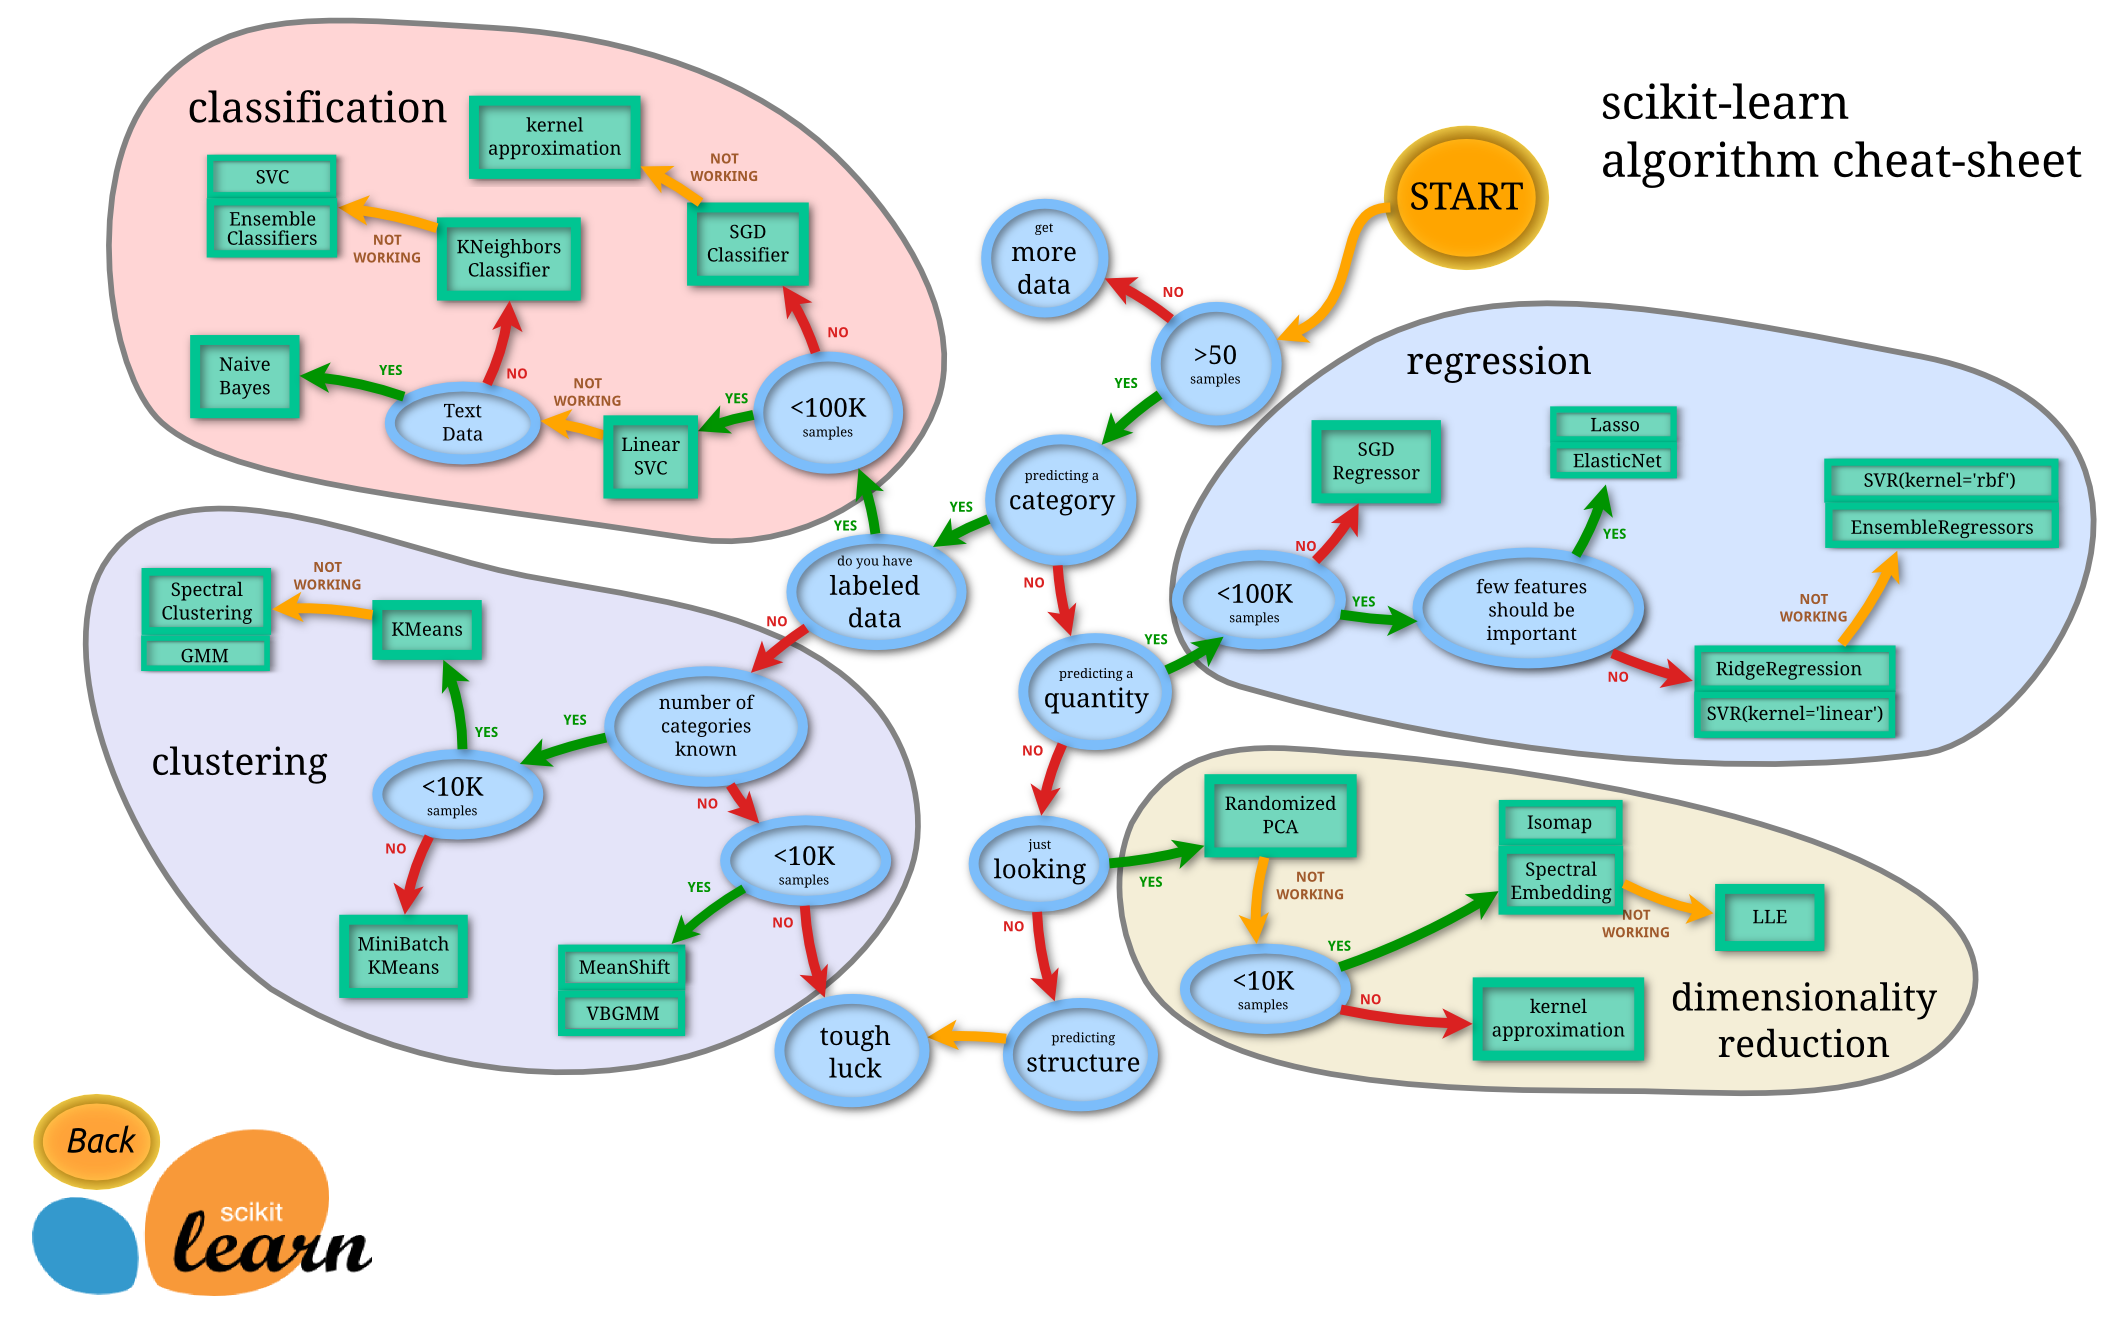
\includegraphics[
	width=0.65\textwidth
	]{images/FlowChartML.png}
	\caption{FlowChartML scikit-learn for any dataset which machine learning algortihm to choose}
	\label{fig:FlowChart}
\end{figure}
%explain the need for automation and then the boost of information, I try to give.

\subsection{research question}
% the proposed annotations
We base our research question on the work of Joaquin to give properties to classifiers\cite{Joaquin-phd}. More specifically we look more closely to the resilience properties and the bias-variance profile. 
Earlier research has been done on scalability and resilience to irrelevant variables\cite{Resil-1}

%\begin{itemize}
%	\item scalability: runtime is measured with either a varying sample size or varying feature space 
%	\item robustness: robustness against irrelevant or redudant features
%	\item robustness: robustness against noisy features
%\end{itemize}

\begin{itemize}
	\item What is the impact on runtime of the amount of features for classification machine learning classifiers?
	\item What is the impact on runtime of the amount of instances for classification machine learning classifiers?
	\item What is the impact on accuracy of irrelevant or redundant features for classification machine learning classifiers?
	\item What is the impact on accuracy of noisy features for classification machine learning classifiers?
	\item What is the percentage of Bias-error or variance-error for classification machine learning classifiers?
\end{itemize}

The question for scalability is how varying sample size and feature space influences the runtime. Is there a measure to match this. 

We rank the classifiers on their performance(predictive accuracy), robustness and scalability to find a ranking like done by Quan Sun and Bernhard Phahringer\cite{ranking}.


%\subsection{thesis structure}


\subsection{Outline}
In the first chapter the research question is introduced. In the second chapter background information is discussed relevant for the research. In the third chapter the setup of the experiments is outlined with the input and output of executed experiments. The fourth chapter shows the results of the experiments. The fifth chapter is a conclusion and discussion of the obtained results. This chapter also explains an outlook on future work and different roads taken. In chapter six the references are outlined. The last chapter is the appendix with some additional information which help with reproducing and validating the results. 
\newpage


\section{Preliminaries} \label{Chapter2}
Before we discuss in detail the solutions for the steps of our approach, this chapter provides
some background knowledge and definitions which are required for a good understanding of
the remainder of this thesis.
\subsection{Sklearn/scikit-learn library}
The scikit-learn library is based in Python and is made to make machine learning in python accessible and organized. 
All resources are open source and hosted on Github. Before scikit-learn there were already other libaries hosting machine learning algorithsm in python but scikit-learn was the first to make a standard guideline which makes the classifier easier to interchange. By having default functions for fitting and predicting.
%subsubsections for classifiers?


\subsubsection{RandomForestClassifier}
RandomForestClassifier is an ensemble method of directive trees \cite{RDF}. During fitting a random forest classifier constructs directive trees on subsamples of the input data and uses the highstest probabilistic prediction for the prediction. These sub-samples are chosen randomly so the results can vary between runs on the same input. A directive tree is a decision tree classifier which splits the features on certain thresholds to decide on the type of class. This splitting of the data is either randomly or choosing the best split, to measure this split a criterion is used like Gini or entropy. The amount of splits, features and samples are also considered and can be inputted. As RandomForestClassifier is made up of trees you can use the ordering of the trees, more specifically the top most layer of the tree to find feature importance. The first split in a decision tree has the most impact on the selection and might indicate a deciding feature. By looking at all the tree in a random forest this gives an average result of important features in a trained dataset.


\subsubsection{KNeighborsClassifier}
In the scikit-learn library KNeighborsClassifier is an implementation of the k-nearest neighbors classification algorithm(kNN)\cite{KNN}. KNN uses instance-based learning or non-generalizing learning. This means that during fitting no complete model is made but only the given feature set is stored in order of appearing. The k-NN uses as it names tells the nearest neighbors for calculation. For prediction the inputted feature set is traversed to find the nearest  k points. Depending on the majority class of the k neighbors the classification is vote is decided. The default metric for distance measuring is Euclidean distance another option is the Manhattan distance which is less accurate but needs less computing. To find the nearest points an option can be made between a ball tree, a kd-tree or a brute search. This can heavily influence the search time, depending on the amount and size of the input (features and instances) this can influence the prediction time heavily but should not influence predictive accuracy. The previously mentioned k parameter is an influencer for prediction quality.\cite{KNN-k}

\subsubsection{SGDClassifier}
SGDClassifier is an incremental function to stochastically approximate the gradient descent of a loss or cost function \cite{SGDClass}. The default classifier to optimize is a linear SVM on its loss function. To fit the classifier it expects continious features with a mean of zero in a sparse setting. This makes the classifier sensitive to categorical data as it performs optimally with continious features. The iterative steps for calculation gradient descent are bounded by the inverse of the learning rate and a threshold value. The threshold value indicates what degree of slope indicates a near minimal or maxima. The learning rate is used to update the model in each iteration. As the fitted functions are linear, if the input has mutliple classes a classifier predicts one class versus all other classes. 

\subsubsection{AdaBoost}
AdaBoost is an ensemble classifier that fits other classifiers and outputs the weighted results of those classifiers \cite{AdaBoost}. AdaBoost trains these other classifiers on previously misclassified results by increasing their influence this makes it heavily subjected to noisy data and outliers. The scikit-learn library uses the multi class AdaBoost-SAMME implementation from J. Zhu et al \cite{MadaB}. The solution of J. Zhu also solves the lack of multi-class solution of the weak learners (other classifiers) by extending the initial AdaBoost classifier with a forward stage wise additive step. In this step a continual calculation of a loss function will output the prediction and in a two class case it reduces to the initial solution.

\subsubsection{SVC-rbf}
SVC-rbf is a support vector classifier(SVC) implementation with a radial basis function. The radial basis function(rbf) is used to handle a large feature dimension, since the standard support vector machine splits the spaces with linearly lines computation grows too large for a large feature space \cite{SVN}. The fit time is already quadratic with the number of samples based on the implementation of libsvm\cite{SVM}. The fitting of a SVC will assign each example to one of two categories and will represent them in a dimension space mapped so there is a clear separation between the two categories. With the radial basis function this is with the distant from the points indicated by a separation area. Classifying a point is finding in which class area this point falls. For a multiclass problem this is done in pairs of two for all categories and then the most voted class is picked \cite{Multi-pair-coup}. To optimize this method there are two main parameters C and gamma. The parameter C trades off misclassification of training examples gainst simplicity of the decision surface, a low C indicates a simple decision surface and lenient misclassification. The gamma parameter is a measure of influence for a single training example. The larger gamma is, the less influence a single instances has.

\subsubsection{GaussianNB}
GaussianNB is a naïve Bayes classifier implementation with the  assumption that the feature set is gaussian distributed \cite{Bayes}. For fitting the data, a partial fit function is used based on the work of Chan, Golub and LeVeque \cite{Sam-var}. This calculates the assumed means and variances of a gaussian distribution of the inputted feature set. Based on this distribution the prediction is made by filling in the maximum likelihood. The limited calculation needed for classification and prediction makes this one of the fastest classifiers. The only parameter of this classifier specifies the prior probabilities of the classes, which will when specified not be adjusted to the given input. 

\subsubsection{BernoulliNB}
BernoulliNB is a naïve Bayes classifier implementation assuming a Bernoulli distribution with Boolean like values \cite{NB-text}. The first step of this implementation is checking if the features are binary-valued, if any other data is found this input will be binarized. This setting can be disabled or reduced by a threshold for the input. Based on this Boolean model a smoothed version of the maximum likelihood is used for prediction. This classifier is mostly used in document classification as it can binary store occurrence useful for prediction class probability.

\subsubsection{GradientBoostingClassifier}
GradientBoost is an ensemble classifier that builds from weaker classifiers \cite{GradientBoost}. Like AdaboostClassifier it builds an additive model in a forward stage-wise fashion.  The weak classifiers used in the scikit-learn implementation are decision trees. The default loss function which is optimized in a stage-wise fashion is a logistic regression for classification with probabilistic outputs\cite{Greedy-GBC}.



\subsection{Definitions and abbreviations}
In this section definitions and abbreviations are explained and set in context. Common synonyms are mentioned to avoid some confusion in text
\subsubsection{Definitions}

\begin{tabular}{ p{0.20\linewidth} p{0.7437\linewidth} }
	
	
	algorithm & A process with a specified in and output that solves a problem in a step by step case.\\ [1ex]
	
	amount & a value that indicates the change of the feature set either in dimension or in value. For \\[1ex]
	
	
	annotations & Adjectives of something like a machine learning classifiers, examples can be robust or biased\\ [1ex]
	
	categorical & property of the features distribution and content of the feature in this case meaning seperate distinc classes, which have no numerical meaning, a unique number for each distinguished class\\ [1ex]
	
	class	 & categorical featueres consist of at least 2 classes\\ [1ex]
	
	datapoint & a datapoint is a single value of a feature. For example an instance has for all feature of a dataset a single datapoint.\\[1ex]
	
	dataset & a dataset are values in a matrix format, where each row represents a single Instance and each collum represent all the values of a feature.\\ [1ex]
	
	dataset manipulation & like the word suggested is the manipulation of a dataset like injecting std deviation or inserting random categories. Adding or removing; of  features or instances to the dataset also counts as it also influences the structure of a dataset. \\ [1ex]
	
	dense matrix & most values in a matrix are different and fluctuate with each row or collumn.(non-zero)\\ [1ex]
	
	distribution & A distribution of a dataset is the probability distribution of that dataset. So considering the dataset what are the odss of picking a specific value. \\ [1ex]
	
	estimator & An estimator is part of an ensemble classifier. It is a single instance of a classifier in the vote of an ensemble classifier.\\ [1ex]
	
	features & part of a whole, Consider a flower it has a color, size, amount of branches, amount of leaves and age. Features describe someone or something in this context it describes something, in this context it is the input to a machine learning for predicting a target , a synonym is variable.\\ [1ex]
	
	fit & To fit the data, synonym with inputting the training data, preparing the classifier for prediction\\ [1ex]
	
	Github & an online platfrom to host data. It uses git commands and is mostly used with programming project to organize a common project which each member can locally alter and centeralizly share updates or modifications. \\ [1ex]	
	
	machine learning classifier & An algorithm that will will learn something and may adopt to the input to better fit the learned instance. To goal of learning can be mostly to predict a Target value, this can be part of an initial input.\\ [1ex]	
	
	numerical & exact values, more uniquely than a category. For example a temperature value or time value. Such a value can be subtracted or divided \\ [1ex]	
	
	profiling & To sketch information of something in a category, so you can relate it to other things in the same category\\ [1ex]
	
	robustness &  The ability of an classifier to cope with changes in features. An classifier is more robust if it deteriorates less than another. \\ [1ex]	
	
	sample & the size of the to be predicted target set. So all distinct features once matched with a target feature\\ [1ex]
	
	scalability & is the capability of a system to handle growing amount of work. \\[1ex]
	
	
	
\end{tabular}
\newpage
\begin{tabular}{ p{0.20\linewidth} p{0.7437\linewidth} }
	slope & a slope value is the value to go from one point to another as a vector. For example from point (1,1) to point (2,3) there is a slope of 1/2.\\[1ex]
	
	sparse matrix & a matrix with lots of zero values, the counterpart of dense were all values fluctuate a lot.	\\ [1ex]
	
	target & In a classificication the value or classes that needs to be predicted, where it mostly about a single feature with at least 2 classes. This can be a feature of something \\ [+1ex]
	
	
	
	weight & The influence or power of a value, function or object. It can be expressed as a fraction of 1 to inidicate its factor from other weights.	\\ [1ex]
	
	
	
	
	
	
	algorithm & \\ [1ex]	
	\end{tabular}

\subsubsection{Abbreviations}
\begin{tabular}{ p{0.20\linewidth} p{0.7437\linewidth} }
	
	adaBoost & adaptive boosting classifier \\
	
	biasVar & bias and variance \\
	
	did & dataset identifier \\
	
	SGD & Stochastic gradient descent \\
	
	std & standard deviation\\
	
	TU/e & Eindhoven University of Technology \\
	
	SVC-rbf & Support vector classification with a radial based function kernel
	
	
\end{tabular}

\newpage
\section{Experimental setup} \label{Chapter3}
For different parts of the research different datasets are chosen. There is overlap between these datasets but the chosen datasets can have a large impact on shown results. Most results are shown as an average result of the datasets involved.

\subsection{MetaFeatures}

\subsubsection{Mean Mutual Information}\label{chapter311}
Meta features like mean mutual information or entropy for categorical features are calculated for our enhanced dataset with duplicate feature and random features. The result is that they do little to change these values and so do not indicate reduced information even tough commonly the results deteriorate when these features are added, seen in figure \ref{fig:MMI}. However if we take the adjusted mean mutual information we can see a more clearer distinction between the permutations of the datasets, figure \ref{fig:AMMI}. With those values the noisy dataset can be more recognized as being worse than before. The normalized seen in figure \ref{fig:NMMI}  is a combination of both which shows depending on the dataset a different ranking of all three datasets.

The calculation of the normalized:
$sqrt(H(labels_true) * H(labels_pred))$


the calculation for two cluster for adjusted mean mutual information:
$AMI(U, V) = [MI(U, V) - E(MI(U, V))] / [max(H(U), H(V)) - E(MI(U, V))]$


The default mutual information is:
$MI(U,V) = \sum_{i = 1}^{I} U \mid\sum_{j = 1}^{I} V \mid \dfrac{\mid U_i \cap V_j\mid}{N} $log $\dfrac{N\mid U_i \cap V_j\mid}{\mid U_i\mid \mid V_j\mid}$
% Misschien een tabel maken en verschil laten zien

\begin{figure}[H]
	\centering
	\begin{subfigure}[b]{0.45\textwidth}
		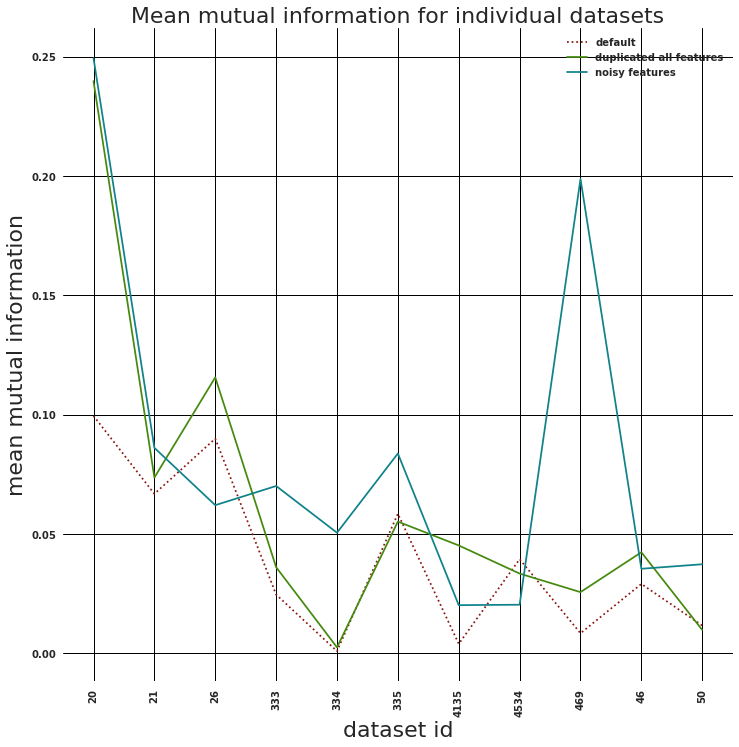
\includegraphics[width=\textwidth]{images/MeanMutualInformation.png}
		\caption{Mean Mutual Information for mututations of datasets}
		\label{fig:MMI}
	\end{subfigure}
	\begin{subfigure}[b]{0.45\textwidth}
		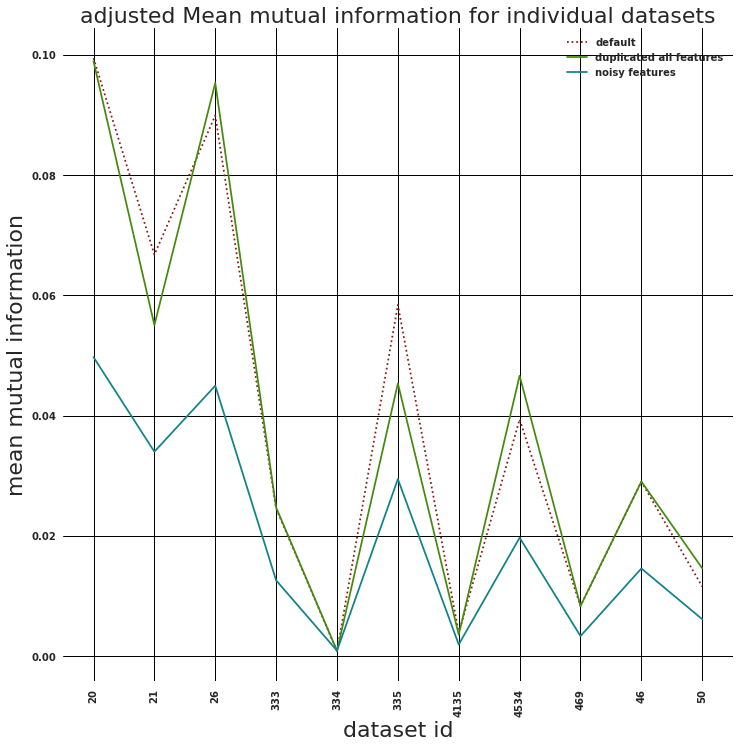
\includegraphics[width=\textwidth]{images/adjustedMeanMutualInformation.png}
		\caption{adjusted Mean Mutual Information for mututations of datasets}
		\label{fig:AMMI}
	\end{subfigure}
	\begin{subfigure}[b]{0.45\textwidth}
		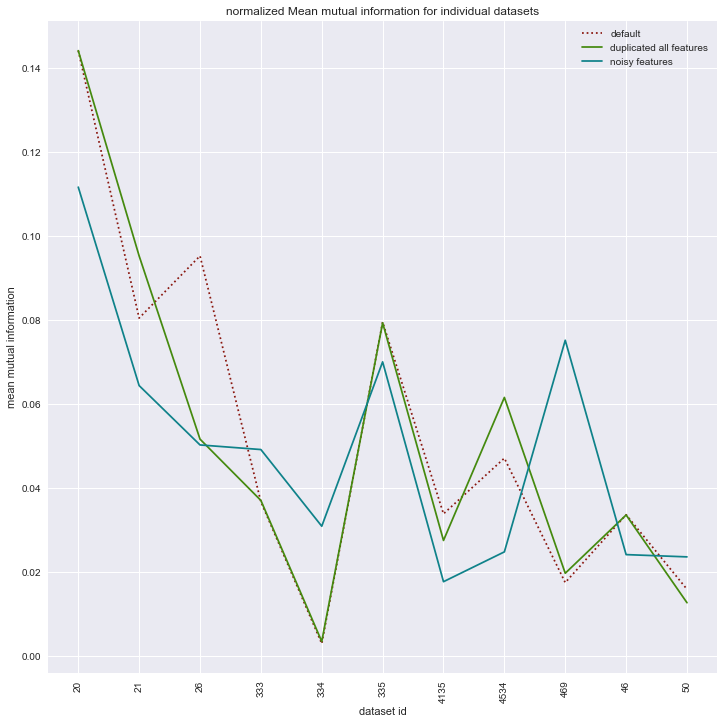
\includegraphics[width=\textwidth]{images/normalizedMeanMutualInformation.png}
		\caption{normalized Mean Mutual Information for mututations of datasets}
		\label{fig:NMMI}
	\end{subfigure}
	\caption{Mutual information difference between measure}\label{fig:MMIs}
\end{figure}

\subsubsection{Feature Importance}\label{chapter312}
Feature importance calculated with a RandomForestClassifer gives an indication what features are important for the ensembled decision trees. In figures \ref{fig:FIC100}, \ref{fig:FIC3}, \ref{fig:FIN100}, \ref{fig:FIN3}, the feature importance of the added random features are shown. This makes it clear that RandomForestClassifier does not recognize these features as unimportant. There is a difference in the perceived importance of random categorical and numerical features. Even more so the distribution of random categorical features. The slope of random categorical with k=3, features importance is also steeper as it more than doubles and for numerical features it only nearly doubles. This is however not true for random categorical features with k= 100 which has an equal absolute increase but starts higher. This can be explained as more perceived variance in k=100 which might indicate better probability of differentiating between the target classes. The lack of increase can be attributed to the cap on the importance at 100$\%$. The original features might give some better results in predicting but the added features still consists of some percentage of the total amount of features. Random Forest Classifier has a limit on the amount of features considered for each split which is capped at a percentage of the total set. This is partly the reason that these random features can be considered as important in the split together with their variance. The variance gives perceived information as you look at a subset of instances the high variability shows that for some target class this feature value is this number and for the other classes the odds of different values for that feature is high. 
\\

In the figures \ref{fig:FIC},\ref{fig:FID} the feature importance of duplicates can be seen. This shows that the order of features is important as the duplicate features have less importance than their percentage of the dataset. It also means that they are not recognized as totally redundant for prediction. The difference between the feature importance for numerical and categorical is also shown. This is partly discussed earlier as the variation in the features and feature order. This has the effect of duplicate numerical features having around 47$\%$ feature importance when the dataset is half duplicates. For categorical featuers this is only 39$\%$. The feature importance of the GradientBoostingClassifier seen in figure \ref{fig:FIGBC} shows a bit less importance for random and duplicate numerical features. The random features even start with more feature importance than the duplicate mostly due to the high variation within the duplicates. With 50$\%$ additional features the duplicates have more importance than the random features on average. 

\begin{figure}[H]
	\centering
	\begin{subfigure}[b]{0.45\textwidth}
		\includegraphics[width=\textwidth]{images/MetaFeatures/FeatureImportanceCat.png}
		\caption{Feature importance for random categorical features with k = 3.}
		\label{fig:FIC3}
	\end{subfigure}
	\begin{subfigure}[b]{0.45\textwidth}
		\includegraphics[width=\textwidth]{images/MetaFeatures/FeatureImportanceNum.png}
		\caption{Feature importance for random categorical features with k = 100.}
		\label{fig:FIC100}
	\end{subfigure}
	\caption{Feature importance of random categorical features. The k value has an impact on the perceived importance of the features.}\label{fig:FIC}
\end{figure}

\begin{figure}[H]
	\centering
	\begin{subfigure}[b]{0.45\textwidth}
		\includegraphics[width=\textwidth]{images/MetaFeatures/FeatureImportanceNum1.png}
		\caption{Feature importance for random numerical features with the default uniform spread between 0 and 1.}
		\label{fig:FIN3}
	\end{subfigure}
	\begin{subfigure}[b]{0.45\textwidth}
		\includegraphics[width=\textwidth]{images/MetaFeatures/FeatureImportanceNum100.png}
		\caption{Feature importance for random numerical features which are multiplied by a 100.}
		\label{fig:FIN100}
	\end{subfigure}
	\caption{Feature importance of random numerical features. The average mean does not influence the importance of random numerical features}\label{fig:FIN}
\end{figure}

\begin{figure}[H]
	\centering
	\begin{subfigure}[b]{0.45\textwidth}
		\includegraphics[width=\textwidth]{images/MetaFeatures/FeatureImportanceNum.png}
		\caption{Feature importance for duplicate features for numerical datasets}
		\label{fig:FIDN}
	\end{subfigure}
	\begin{subfigure}[b]{0.45\textwidth}
		\includegraphics[width=\textwidth]{images/MetaFeatures/FeatureImportanceCat.png}
		\caption{Feature importance for duplicate featueres for categorical datasets.}
		\label{fig:FIDC}
	\end{subfigure}
	\caption{Feature importance of duplicate features and their effect on categorical or numerical datasets}\label{fig:FID}
\end{figure}
\begin{figure}[h] 
	\centering
	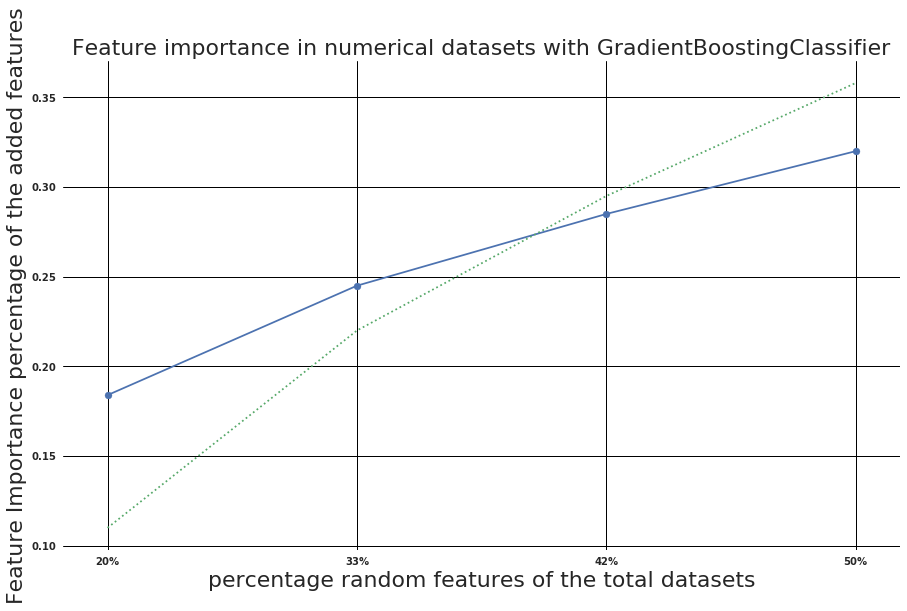
\includegraphics[
	width=0.65\textwidth
	]{images/MetaFeatures/featureImportanceGBC.png}
	\caption{Feature importance for duplicate features and random features calculated with a GradientBoostingClassifier instead of the RandomForestClassifier on a numerical dataset}
	\label{fig:FIGBC}
\end{figure}


\subsection{Model Validation strategies}
What strategies do we use to split the datasets into training and test to measure predictive accuracy, duration, bias and variance.
\subsubsection{Cross validation} \label{cross-val}
To easily test a single dataset once we use cross validation as it does this k times to get k splits of equal size. We can observe k classifications, to gain insight in duration time. We pick k=10 as standard as it is perceived to be a well rounded amount of folds for decent results\cite{Cross}.

\subsubsection{Bootstrapping} \label{motivation}
For the bias variance calculation it is import to gain multiple predictions for the same instance and with bootstrapping this can be easily achieved. The downside however can be an increased bias and reduced variance error.  

\subsection{Datasets} \label{description}
Depending on the property we are going to study we need different datasets or can make assumption. Classification features are not an optimal input for a nearest neighbor classifier as the distant between converted numbers does not tell much about the relation between the features. Multiple target classes datasets are inconvenient for the bias-variance calculation, so we focus on 2 class target datasets, which there are plenty enough on openml. 

\subsubsection{Bias-variance datasets}
An important part of a dataset to be viable for bias variance analysis is it having 2 classes as target. This is due to calculation we use to find the bias and variance error. The bias and variance error is in this way like recall or precision error more suitable for a 2 classes target.  %give picture of instance versus features
\subsubsection{Categorical datasets}
Categorical datasets hold only features with categorical values. These features are useful for a RandomForestClassifeir to make decisisons with the internal decision tree but for a KNeighborsClassifier it is harder to use these features as input as the structure of the translation to numbers also has an effect.
\subsubsection{Numerical datasets}
Numerical datasets hold only features with numerical values. These features are hard to use by classifiers like BernoulliNB which translates the values in their own way by uniqueness. For classifiers like KNeighborsClassifier it is easier to use the uniquess of numerical values for predictions.

\subsection{Collected data}
For each experiment data is saved to give insight to what the results are. Depending on the experiment different data is important or stored. 
\begin{itemize}
	\item predictive accuracy for measuring the predictive accuracy we store the default sklearn scoring calculation
	\item duration instances for the time needed to calculate 
	\item control data like predictions and real target values. Summarizing data of the predictions to make a faster observation. 
\end{itemize}
\subsubsection{Duration}
For each classification instance and for each prediction the time is added to indicate how the classification took. 

\subsubsection{Predictions}\label{pred}
For each predictions the outputted target value. Multiple files indicate multiple predictions. One of the files is also the true prediction of the inputted test set. 

\subsubsection{scores}
Gives the predictive accuracy of all the made classifiers. There can be multiple lists for each configuration of classifier or test input. The score is a value between 0 and 1 indicating the fraction of rightly predicted values

\subsubsection{SummaryGuesses}
SummaryGuesses give a quick overview of the obtained results. It stores in python dictonaries the total amount of predictions for each class. The results is that you can easily observe if a classifier has picked a class exclusively and you can compare the balance to the inputted dataset to see if the classifier does find a difference between classes. This data can also be generated from the predictions \ref{pred}.

\subsubsection{BiasVar}
When bootstrapping is done a bias and variance error is calculated together with the total error value. These are stored for easy lookup to the bias and variance error part of a classifier.

\subsubsection{Identifier}
The data input is shuffled as the saved datasets are sorted by class. The identifier can be used to match prediction results to a specific instance in the dataset. This way of saving is used to reduce space needed to save potential useful information. Odd behavior on small datasets can be explained by an off balanced dataset for training. The split of the data can be realistic but may affect averaged result significantly. 

\subsubsection{RemovedFeatures}
In the case we use metafeatures like feature importance or correlation to remove features we save the removed features per fold of the cross validation. Comparing the removed features of each fold we can find if there are multiple irrelevant features or the features are likely to be randomly more important than another.

\subsection{Experiments}
Experiments are grouped by all mentioned classifier with some initial settings on the dataset and/or classifiers. Experiments are defined as functions in python with input values indicating the way the experiment is done and on which dataset.
\subsubsection{Scalability}
Scalability experiments can be split up in instance based or features based. To measure the effect of features we take datasets with lots of features and remove features in steps to find the impact of these lost features. There is a disadvantage with this strategy as some classifiers calculate values like feature importance which depend on a somewhat complete dataset of features. The removed features are randomly chosen and can be defining features for the accuracy of the dataset. 

To combat this we also do feature removing based on feature importance of a RandomForestClassifier and on correlation between features. For feature importance we train a RandomForestClassifier to find the most important features. We then remove the least important features and remember the features we removed to also remove them in the test set. For correlation we find the feature the 2 most correlated features and then remove the feature that is most correlated to all features of the 2. Based on the amount we are going to remove we repeat the process to remove more.


Another option  to measure scalability is to measure the impact of number of instances. For most classifiers each instance is considered during training and we measure an average calculation for each feature. The duration is measured over the whole dataset by doing a 10 fold cross validation.
%We compare the found scalability against the perceived running time upper or lower bounds. 

\subsubsection{Duplicate features}
Duplicate features experiments have multiple goals in mind. By adding existing feature we can measure scalability of datasets with some amount of features. These duplicate features can also be identified as adding little to the dataset or the same features can overrule existing important features. The accuracy on these modified dataset
can teach us about the impact of features on accuracy and how classifiers handle these irrelevant features. The method to add these duplicate features is by randomly picking and adding. This can result in features being multiple times in the manipulated  dataset even though it is only twice the orignal dataset size. The accuracy is measured over the whole dataset by doing a 10 fold cross validation.

\subsubsection{Random Features}
Random features experiments have similar goals in mind as duplicate features. By adding the random features we can measure scalability of datasets with randomish features. These random features can deceivingly have information as there is much variability. By measuring the accuracy we can observe what the impact is for different classifiers. There are two sorts of random features we add; Numerical and categorical features. We add either the categorical or numerical depending on the distribution of the dataset. The odds of either a categorical or numerical feature being added is the distribution of the initial dataset. The accuracy is measured over the whole dataset by doing a 10 fold cross validation. %\cite{catVSnum} the influence of categorical vs numerical why we need to add a similair feature.


 
\paragraph{categorical random features \newline}
The categorical random feature is a uniform value between 0 and k. The value of k can influence how a classifier perceive this random feature. For all the instances in the set a uniform random number between 0 and 1 is multiplied by k and then rounded. 
\paragraph{numerical random features \newline}
The numerical random feature is a uniform random value between 0 and 1. This feature has in this case all unique values.

\subsubsection{Redundant duplicate features}
Redundant duplicate features experiments are datasets with duplicate features appended in training and different features appended to the test set. These features so appear to have some predictive quality similair to the features already in the dataset. These features are similair to the original dataset, so we can better measure the impact of scalability of features similair to the duplicate features. The comparison can be made to the randomly added features datasets in terms of scalability and predictive accuracy 


\subsubsection{Noisy data}
Datasets can get more noisy over time. During training of a machine learning classifier the dataset is clean and over time new data can change. By measuring the predictive accuracy off the classifiers on more noisy datasets the robustness can be measured. The accuracy is measured over the whole dataset by doing a 10 fold cross validation.

\paragraph{categorical features \newline}
To explain the implementation of our noisy data for a categorical feature we present this snippet of pseudo code. THe input is the dataset X and the amount of noise. The amount can be converted to a percentage of features being flipped by this formula $()1-1/(amount+0.5))*100$. The distribution$_X$ is derived from the dataset X as the probability distribution of all categorical classes in a feature. The random.choice function uses this probability function to pick a value in the range of the feature. The default random function picks a uniform random value between 0 and 1.  \\
Initiliaze distribution$_X$ for all features in dataset X\\
\textbf{for} numerical feature k in dataset X\\
.\hspace{1cm} \textbf{for} datapoint x in feature k\\
.\hspace{2cm} \textbf{if} random()*amount $>$ 0.5 \\	
.\hspace{3cm} x = random.choice(distribution$_X$ feature k) 
\\

\paragraph{numerical features \newline}
The input is the dataset X and the amount of noise. The amount is multiplied by the standard deviation to give the maximum deviation of the feature. The calculation for the std$_X$ is done beforehand to control the deviation for all datapoints in the feature set. The random function is like mentioned before producing a uniform random value between 0 and 1.\\
Calculate std$_X$ for all features in dataset X\\
\textbf{for} numerical feature k in dataset X\\
.\hspace{1cm} \textbf{for} datapoint x in feature k\\
.\hspace{2cm} \textbf{if} random() $>$ 0.5 \\	
.\hspace{3cm} x = x + random() *amount*(std$_X$ for feature k)\\
.\hspace{2cm} \textbf{else}  \\	
.\hspace{3cm} x = x - random() *amount*(std$_X$ for feature k) 
\\

\subsubsection{Bias Variance}
To measure the bias and variance error factor we use the calculation of Kohavi and Wolpert\cite{BiasCalc}. This is the same measure used in the work of Joaquin et al.\cite{Bias-var}. This experiment is made to reproduce that experiment with the scicikit-learn library. The input for the bias and variance calculation is done by doing 40 bootstraps. 

\subsubsection{PreProcessing}
Preprocessing is a neccesary job for most machine learning classifiers as they are dependent on the input structure to classify. For example KNeighborsClassifier is dependent on distance between instances, if we look at categorical data the distance between instances is not always relevant. That is why experiments with specifically categorical datasets are repeated with some preprocessing for at least KNeighborsClassifier, SGDClassifier and SVC-rbf. For these classifiers a translation of categorical features seems to be neccesary \cite{KNN-Sym}\cite{SVM-sym}. The proposed preprocessing steps are OneHotEncoder and Standardscaler in that order. OneHotEncoder translates the categorical features in features corresponding to the amount of classes. Each feature is then a boolean value of being the class or not. The StandardScaler removes the mean and scales on the standard deviation. Storing the mean and std of the training set to use it to transform the test set balances the dataset accordingly. 
\newpage
\section{Experimental Results} \label{Chapter4}


\subsection{Scalability}
All results with a duration axis. The duration axis is in seconds and shows a 10 fold cross validiation. This means that the duration encompasses 10 times fitting over 90\% of the data and 10 times predicting 10\% of the data.

\subsubsection{features}
Due to the robustness experiments a lot of results change the composition of a dataset in the feature dimension. In this subsection all results changing the composition of a dataset are included with a duration y axis. 



\paragraph{Added features}
In figures \ref{fig:SADRC},\ref{fig:SADRP},\ref{fig:SADR} the durations of adding redundant duplicate or random features are shown. In figures \ref{fig:SADRC2},\ref{fig:SADRP2},\ref{fig:SADR2} the durations of adding duplicate or random features are shown In figure \ref{fig:SADRC} the classification times are shown for a growing feature size, these durations are a great part of most classifiers.In figure \ref{fig:SADRP} the prediction time is shown, here most classifier take only a short while. The combined time can be seen in figure \ref{fig:SADR} which shows the total difference.
The averaged size of this dataset is 3797 instances and 200 features.  and the slope of these added figures is seen in figure \ref{fig:SADS}.
\begin{figure}[H]
	\centering	
	\begin{subfigure}[b]{0.45\textwidth}
		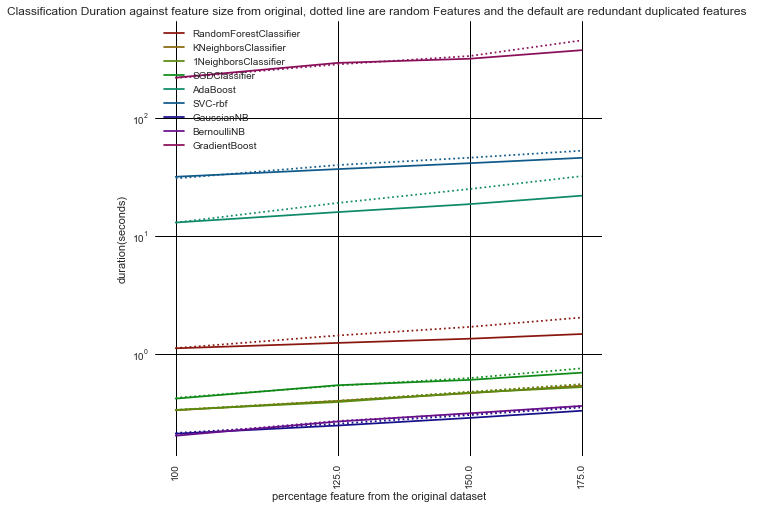
\includegraphics[width=\textwidth]{images/scalability/FeatAddDupRandClass.png}
		\caption{only the time needed to predict }
		\label{fig:SADRC}
	\end{subfigure}
	\begin{subfigure}[b]{0.45\textwidth}
		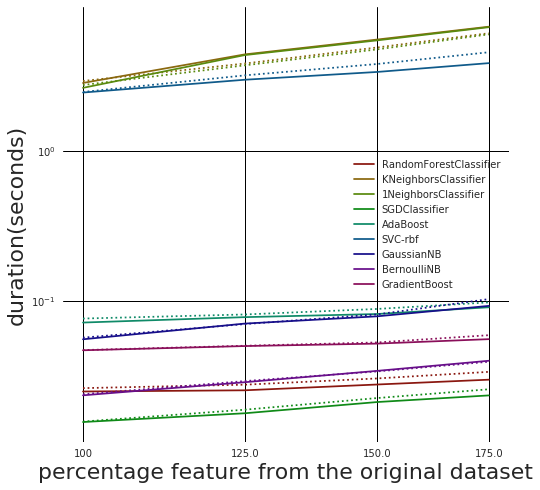
\includegraphics[width=\textwidth]{images/scalability/FeatAddDupRandPred.png}
		\caption{only the time needed to make the predictions}
		\label{fig:SADRP}
	\end{subfigure}
	\begin{subfigure}[b]{0.45\textwidth}
		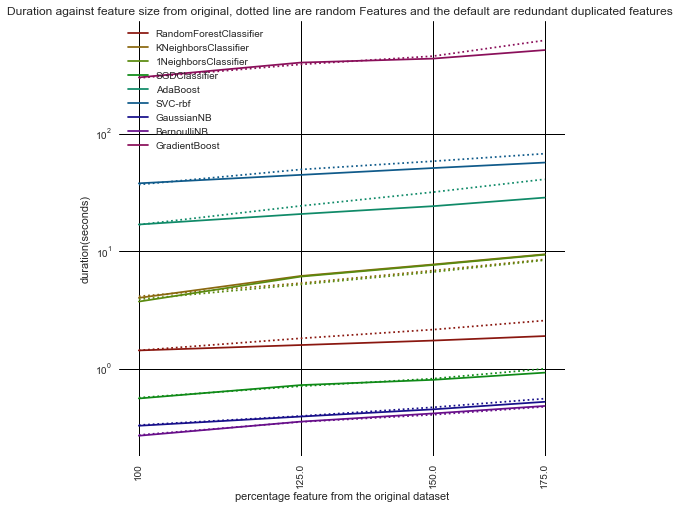
\includegraphics[width=\textwidth]{images/scalability/FeatAddDupRand.png}
		\caption{The combined time of predicting and classifying on a dataset with added random and redundant duplicated features}
		\label{fig:SADR}
	\end{subfigure}
	\caption{Adding redundant duplicate and random features to a dataset plotted against the duration needed.}
	\label{fig:ScalableAdded}
\end{figure}
\begin{figure}[H]
	\centering	
	\begin{subfigure}[b]{0.45\textwidth}
		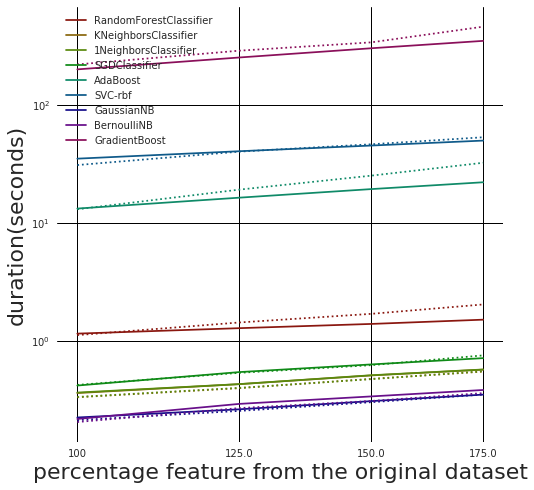
\includegraphics[width=\textwidth]{images/appendix/FeatAddDupRandPredClass.png}
		\caption{only the time needed to predict }
		\label{fig:SADRC2}
	\end{subfigure}
	\begin{subfigure}[b]{0.45\textwidth}
		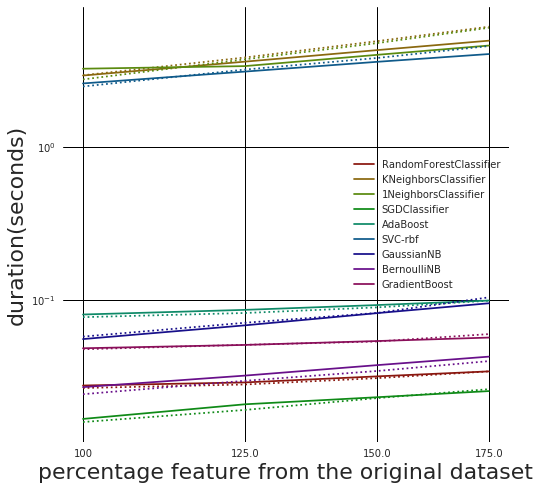
\includegraphics[width=\textwidth]{images/appendix/FeatAddDupRandPred.png}
		\caption{only the time needed to make the predictions}
		\label{fig:SADRP2}
	\end{subfigure}
	\begin{subfigure}[b]{0.45\textwidth}
		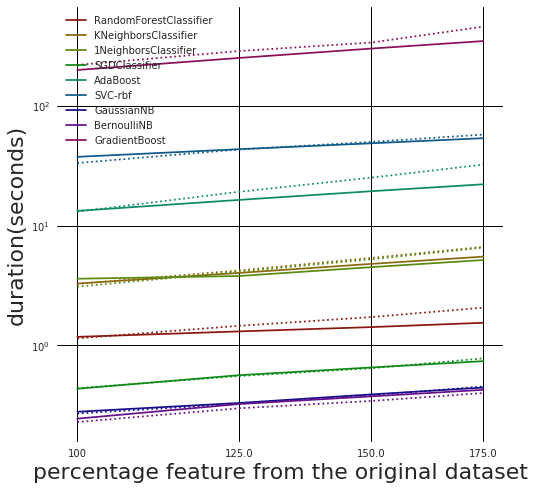
\includegraphics[width=\textwidth]{images/appendix/FeatAddDupRand.png}
		\caption{The combined time of predicting and classifying on a dataset with added random and  duplicated features}
		\label{fig:SADR2}
	\end{subfigure}
	\caption{Adding duplicate and random features to a dataset plotted against the duration needed.}
	\label{fig:ScalableAdded2}
\end{figure}


\begin{figure}[h] 
	\centering
	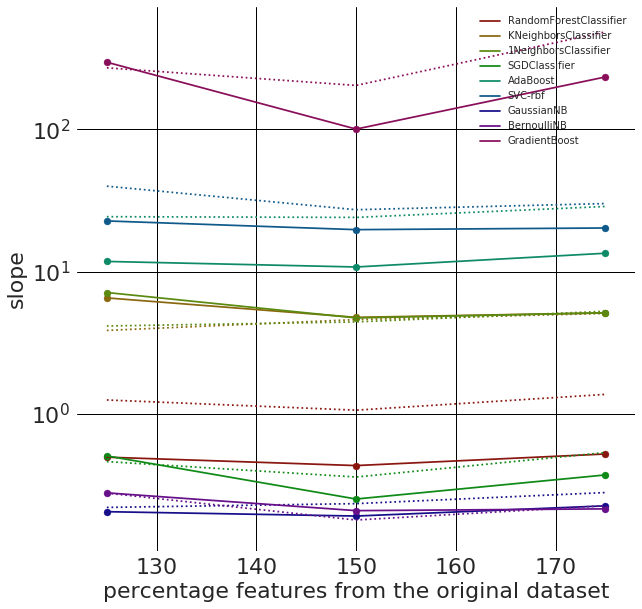
\includegraphics[
	width=0.65\textwidth
	]{images/scalability/FeatAddDupRandSlope.png}
	\caption{Slope for \ref{fig:SADR} with the dotted line for random added features and the straight line for redundant duplicate features}
	\label{fig:SADS}
\end{figure}



\textbf{RandomForestClassifier} The duration of the RandomForestClassifier is fairly below average in comparison. The difference between random and redundant duplicate is noticable as the random feature take more time mostly for classification as classification takes the longest of the two. This longer duration can be attributed to the at. As seen in section\ref{chapter312} the features are given some importance which will take some time. There is also hardly any difference between the redundant or normal duplicate features.  \\

\textbf{KNeighborsClassifier} The duration of KNeighborsClassifier is average in comparison. Most of the time is needed for prediction as there is only minimal effort during classification. The difference in prediction time between the three variants is supringly large. The smallest predicition duration is for the duplicate features which seems obvious considering they are most similair to the features in the training set. The redundant duplicate features take longer than the random which can be explained as slightly more variation between the features. On average the std of a random numerical feature is 0.28, the std of a numerical redundant features is higher on average in for each dataset. A difference between 1NN and kNN is also only minimal as the largest part of the prediction is making for example a kd-tree and the search on such a data structure is far smaller than the making of.\\

\textbf{SGDClassifier} SGDClassifier has one of the shortest durations of the machine learning process. The prediction is even the smallest. There is also hardly any difference between the input of features. The random features have take only  a slighly longer than any sort of duplicate feature. The short prediciton time is due to only filling in made linear regressions lines based on the inputted features. \\

\textbf{AdaBoost} AdaBoost has one of the longest classification times with defaultly 5 times more estimators it is bound to take some more time as RandomForestClassifier. The impact of random features compared to any sort of duplicate features is large with a steady increase in duration. This is mostly due to the variation in the added features and the more effort the Decision Trees need to filter out any information. The effect of the adaptive boost is unnoticable between random or duplicate features compared to the standard RandomForestClassifier.  \\

\textbf{SVC-rbf} SVC-rbf has one of the slowest classification and prediction time. With the calculation of the decision surface taking the most time. The duration of prediction is also slow in comparison to the other classifiers. The impact of the random features is noticibale with the variation present in those features SVC takes a bit longer to  classifiy and predict. \\

\textbf{GaussianNB} GaussianNB has one of the quickest prediction and classification time. The calculation needed for the mean and the variance is easy and there seems no significant impact of the different added features. That is reasonable as it should have little impact on the calculation of the mean and variance of a single feature.\\

\textbf{BernoulliNB} BernoulliNB is also one of the quickest in prediction and classification time. With a similair approach as BernoulliNB there is little calculation in both prediction and classification. The only added calcualtion for BernoulliNB is a binarization. \\

\textbf{GradientBoostingClassifier} The GradientBoostingClassifier takes the longest amount of time of all classifiers. With 10 times the estimators of RandomForestClassifier it takes on average 250 times the total duration. With the calculation in multiple stages the duration time ramps up to fit the Decision trees. The impact of random features is more than either of the duplicate features. This is also due to more variation in the features with also using DecisionTrees, GradientBoostingClassifier %TODO feature importance of GradientBoostingClassifier
  \\

The slopes of the different classifiers are close to a linear scale and vary a bit between addition(figure \ref{fig:SADS}). This is mostly an the starting impact of the added features compared to the clean dataset. 


\paragraph{Removed features}
In figure \ref{fig:FeatRem} the duration against features removed from a dataset are shown. Three different techniques of feature removing are shown. In figure \ref{fig:FeatRemImp} features are randomly remove or a RandomForestClassifier is fitted on the training set and the least important feature is removed. In figure \ref{fig:FeatCorImp} the features are removed by their importance or by having the most correlation with another feature in the training set. In figure \ref{fig:FeatRemImp} the average dataset is 2230 instances with 307 features and in figure \ref{fig:FeatCorImp} the average dataset is 3329 instances with 258 features.
\begin{figure}[H]
	\centering	
	\begin{subfigure}[b]{0.45\textwidth}
		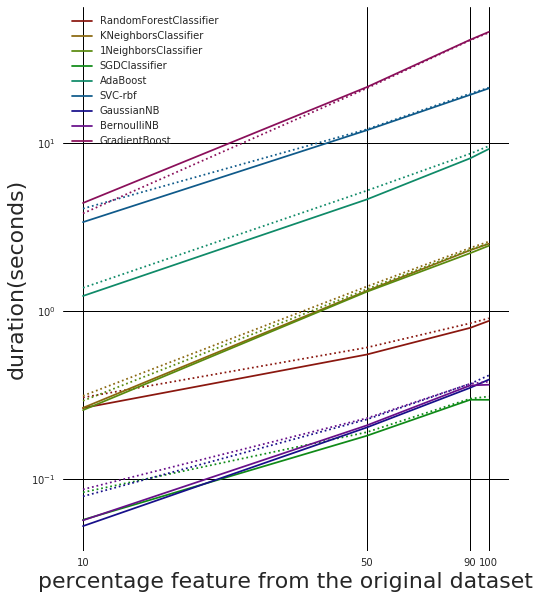
\includegraphics[
		width=0.65\textwidth
		]{images/scalability/FeatRemImp.png}
		\caption{features randomly removed or removed by importance }
		\label{fig:FeatRemImp}
	\end{subfigure}
	\begin{subfigure}[b]{0.45\textwidth}
		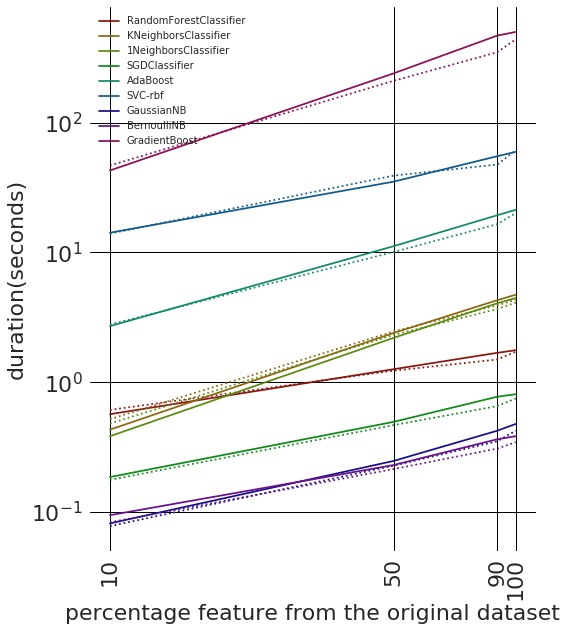
\includegraphics[
		width=0.65\textwidth
		]{images/scalability/FeatCorImp.png}
		\caption{features removed by least importance or by most correlation with other features}
		\label{fig:FeatCorImp}
	\end{subfigure}
	
	\caption{Duration of classification and prediction of the classifiers against removing features from clean datasets.}
	\label{fig:FeatRem}
\end{figure}

\textbf{RandomForestClassifier} A small difference in duration can be seen between the randomly removed feature and feature removed by lack of importance. On the smallest dataset the importance removed feature dataset takes longer. This can be explained as the feature set needing more time for the quality of the split. Between highest correlation removing and importance removing the difference is minimal\\

\textbf{KNeighborsClassifier} For KNeighborsClassifer there is also more time needed for a small importance removed dataset and even more for highest correlation based removing. The longest duration for correlation based removing can come from the lack of correlation giving more variation between features as they are least similair to each other. This means that the features are different and more calculation is needed to find neighbors. For important features this is also the case but to a lesser extend than the least correlated features, which indicates that some features can still be closesly correlated but still have some perceived importance.\\

\textbf{SGDClassifier} The SGDClassifier can be seen as one of the quickest algorithms in figure \ref{fig:FeatRemImp} but a bit more time consuming in figure \ref{fig:FeatCorImp}. There is even a big time difference between randomly removing features and removing feature by least importance. The more important the features the longer the classifier needs. This can be explained as the features less likely being standard for the input of the classifier. This means that the important featuers are likely dense features. \\

\textbf{AdaBoost} AdaBoost classifier needs more time for least important removed feature dataset than randomly removed features. This seems similair to the RandomForestClassifier. With the important features left AdaBoost has a harder time to classify outliers which the removed features were more likely to be used for. \\

\textbf{SVC-rbf} The SVC-rbf classifier needs more time for important feature in line with most other classifier, this means that with the less important feature removed, more time is needed for the decision surface calculation. This is also in line with the similairty of duration between the feature importance and correlation features being removed duration. With less correlated features being important features the odds are higher of a less linear relation between the targets. \\

\textbf{GaussianNB} Removing the least important features from a dataset has less of an impact of decreasing the duration than removing random features. The effect of calculating means and variances should not have this effect as that calculation is more dependent on instances than values. The only reason can be the calculation of the maximum likelihood needing slightly more workload. The Difference between feature importance and correlation feature removing is negligible \\

\textbf{BernoulliNB} The same behavior seen in the GaussianNB can be seen for the BernoulliNB. This can be due to the randomly remaining features being easier to binarize. As that is the only factor that might be influenced by values of the features. \\

\textbf{GradientBoostingClassifier} As the only classifer GradientBoostingClassifier takes less time with only the most important features. This can be the nature of the stagewise steps of GradientBoostingClassfier needing less time with more important features than random features whos importance can be questionable. The dataset with the least correlated features hardly as any difference with the least important removed feature dataset.\\


\paragraph{combined}
in figure \ref{fig:FeatManLog} adding and removing features is shown.
in figure \ref{fig:SlopeDurMan} the slopes are shown for adding and removing the features. The two different calculation styles show what the difference in measuring has for influence. Figure \ref{fig:FeatManSlope1Log} has the most balanced approach as basing the calculation on the clean dataset reduces the influence of outliers. The slopes in figure \ref{fig:SADS} are also considered in these results.

For most classifiers the results paint a clear picture. Removing features has more impact on duration as adding additional features, the general trendline is mostly linear for adding features and less linear for feature removing. In figure \ref{fig:FeatManSlope1Log} there is a decrease of the duration slope from the minimal to the clean dataset. Averaging these results gives a slope close to the slope found in only adding features. Another strange behaviour is around the full dataset results there is a drop in the slope. For SGDClassifier there is nearly no difference in duration between 90$\%$ and 100$\%$ features of the dataset seen as the slope dropping outside of the picture. For most classifiers there is a similair but less drastic drop. The drop can be seen in figure \ref{fig:FeatManSlope1Log} as being low. This is because the difference between instances is small and the duration calculcation is inaccurate. With the short duration needed needed for training and prediction in the SGDClassifier the difference can be larger between the results. 

\begin{figure}[H]
	\centering	
	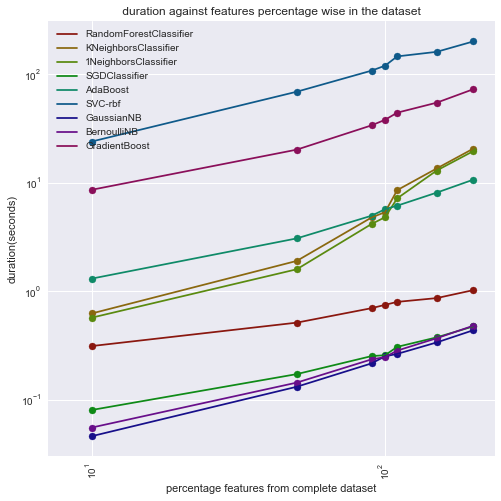
\includegraphics[
	width=0.65\textwidth
	]{images/scalability/FeatManLog.png}
	\caption{features removed randomly and features  redundantly duplicated slope }
	\label{fig:FeatManLog}	
\end{figure}
\begin{figure}[H]
	\centering	
	\begin{subfigure}[b]{0.45\textwidth}
		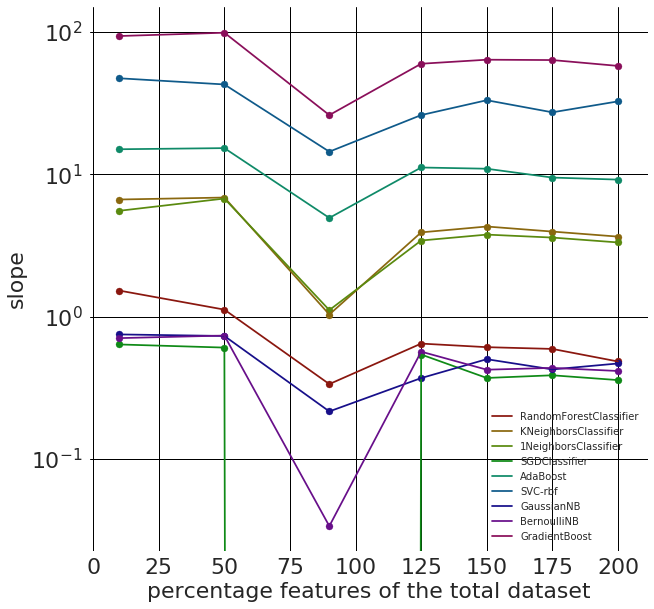
\includegraphics[
		width=0.65\textwidth
		]{images/scalability/FeatManSlopeLog.png}
		\caption{features removed randomly and features   duplicated with a log scale }
		\label{fig:FeatManSlopeLog}
	\end{subfigure}
	\begin{subfigure}[b]{0.45\textwidth}
		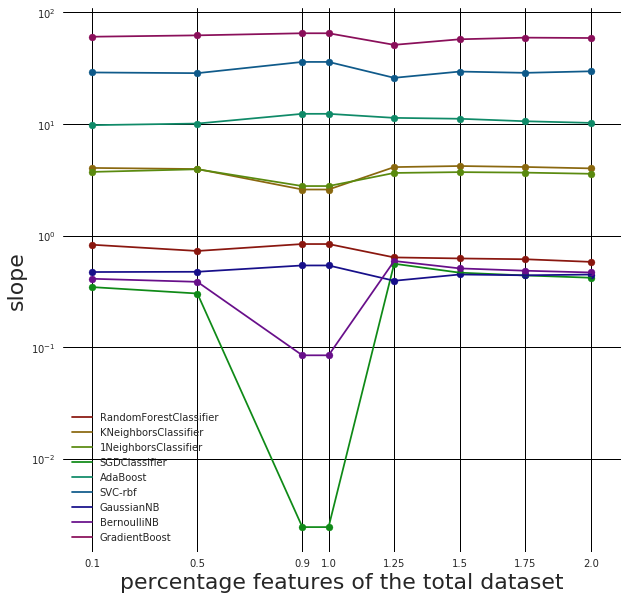
\includegraphics[
		width=0.65\textwidth
		]{images/scalability/FeatManSlope1Log.png}
		\caption{features removed randomly and features   duplicated slope based on the average point of a clean dataset, with a log scale}
		\label{fig:FeatManSlope1Log}
	\end{subfigure}
	
	\caption{Slopes of Feature percentage total duration of the original dataset calculated from figure \ref{fig:FeatManLog}.}
	\label{fig:SlopeDurMan}
\end{figure}




\newpage
\subsubsection{Instances}
\begin{figure}[h] 
	\centering
	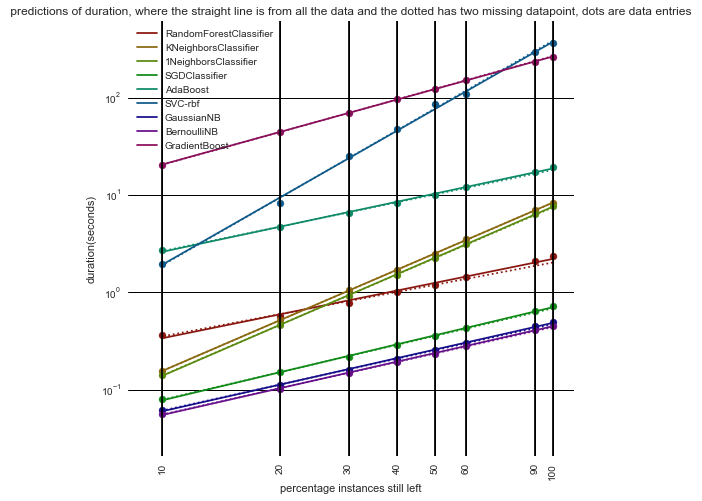
\includegraphics[
	width=0.65\textwidth
	]{images/scalability/Instances.png}
	\caption{The dataset is reduced to a split of the initial dataset and then cross validation is done on the reduced dataset. The lines are predictions}
	\label{fig:Instances}
\end{figure}

\begin{figure}[h] 
	\centering
	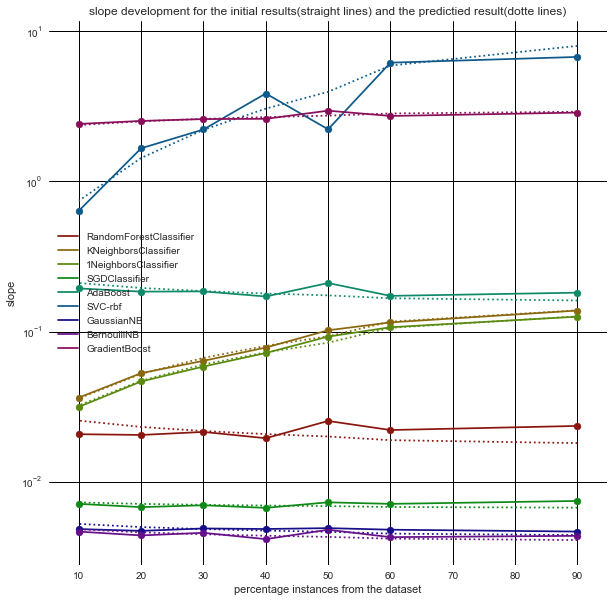
\includegraphics[
	width=0.65\textwidth
	]{images/scalability/InstancesPredictionSlope.png}
	\caption{The slopes are calculated from the results in \ref{fig:Instances} }
	\label{fig:InstancesPredSlope}
\end{figure}

\begin{figure}[h] 
	\centering
	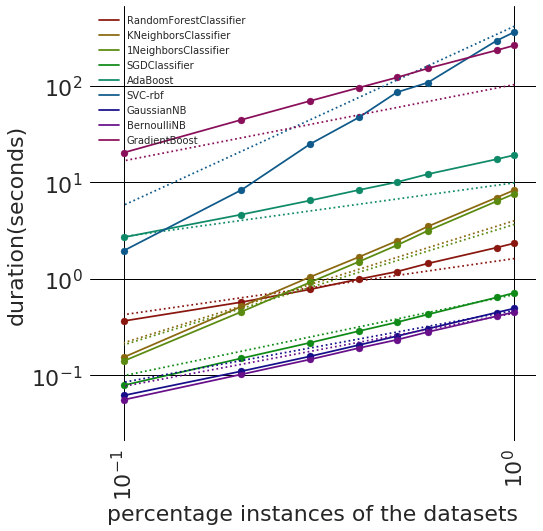
\includegraphics[
	width=0.65\textwidth
	]{images/scalability/InstancesPrediction.png}
	\caption{the dataset is reduced to a fraction of the initial dataset. A prediction is made of the duration of classification and prediction per dataset, indicated by the dotted line }
	\label{fig:InstancesPred}
\end{figure}



\textbf{RandomForestClassifier} \\
\textbf{KNeighborsClassifier} \\
\textbf{SGDClassifier} \\
\textbf{AdaBoost} \\
\textbf{SVC-rbf} \\
\textbf{GaussianNB} \\
\textbf{BernoulliNB} \\
\textbf{GradientBoostingClassifier} \\

\paragraph{Prediction}
For scalability it is easier to predict then for accuracy. The lines for the duration increase are on a log scale nearly linear. This makes for an easy fit with a linear line with log preprocessing. In figure \ref{fig:Instances} you can see that the averaged results of an instance scalability has a good fit. However if we try to predict on an individual bases per dataset the results are less promising(figure \ref{fig:InstancesPred}). Here we tried fitting a KernelRidge with some additional meta features. The meta features include the number of instances,features,numeric features ,categorical featueres and number of classes. 

\newpage
\subsection{Redundant features}
This section focusses on feature manipulation of clean datasets and the accuracy impact. By either removing or adding features the dataset changes and maybe also the workings of classifiers. By comparing the results of a clean dataset to a manipulation in the feature dimension we see how classifiers handle these feature changes.

\subsubsection{Adding features}
We consider here random, duplicate and redundant duplicate features as they are all redundant. In section \ref{chapter312} the importance and in section \ref{chapter311} the mutual information is shown which changes with the addition of certain features.\\

\begin{figure}[H]
	\centering	
	\begin{subfigure}[b]{0.45\textwidth}
		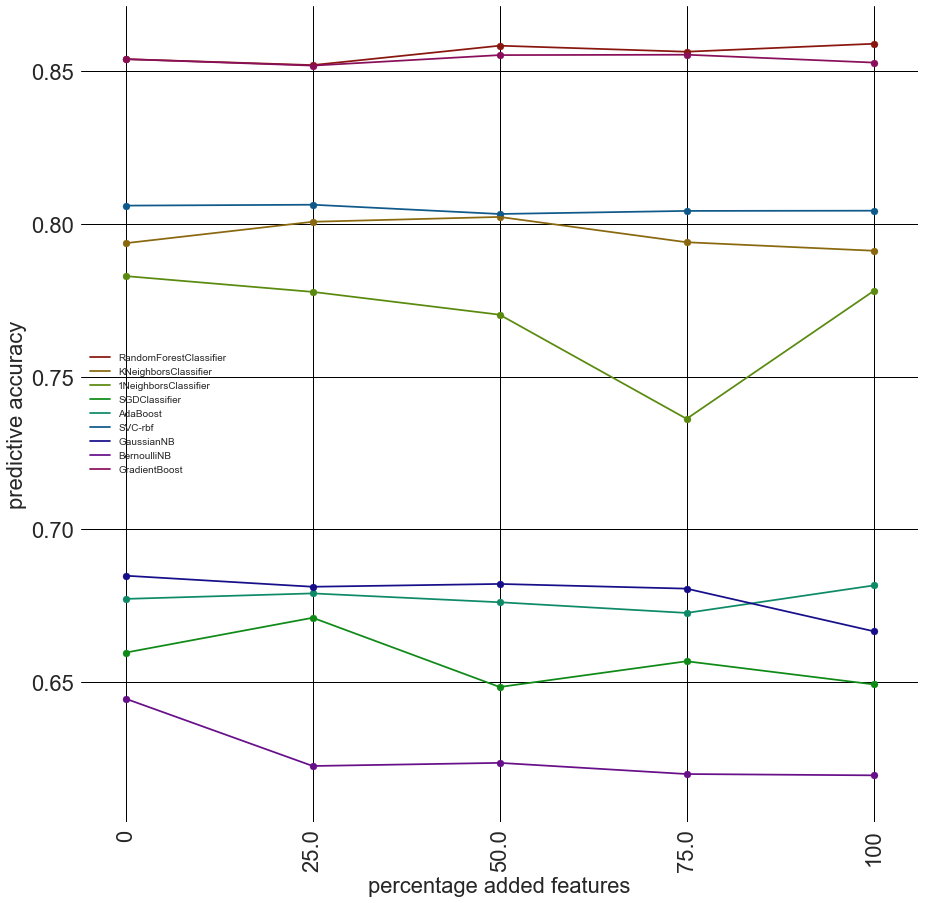
\includegraphics[
		width=0.65\textwidth
		]{images/RedudantFeature/predAddCatDup.png}
		\caption{Adding increasingly more duplicate features to categorical datasets}
		\label{fig:predCatDup}
	\end{subfigure}
	\begin{subfigure}[b]{0.45\textwidth}
		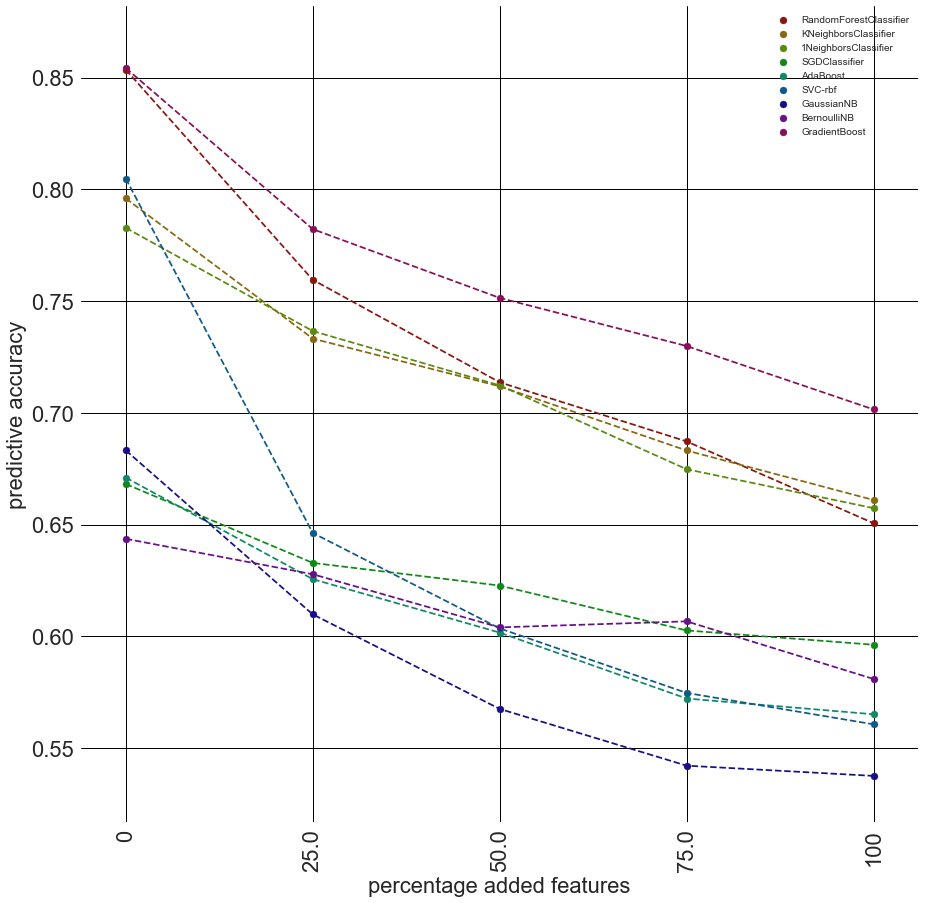
\includegraphics[
		width=0.65\textwidth
		]{images/RedudantFeature/predAddCatReDup.png}
		\caption{Adding increasingly more redundant duplicate features to categorical datasets}
		\label{fig:predCatReDup}
	\end{subfigure}
\begin{subfigure}[b]{0.45\textwidth}
	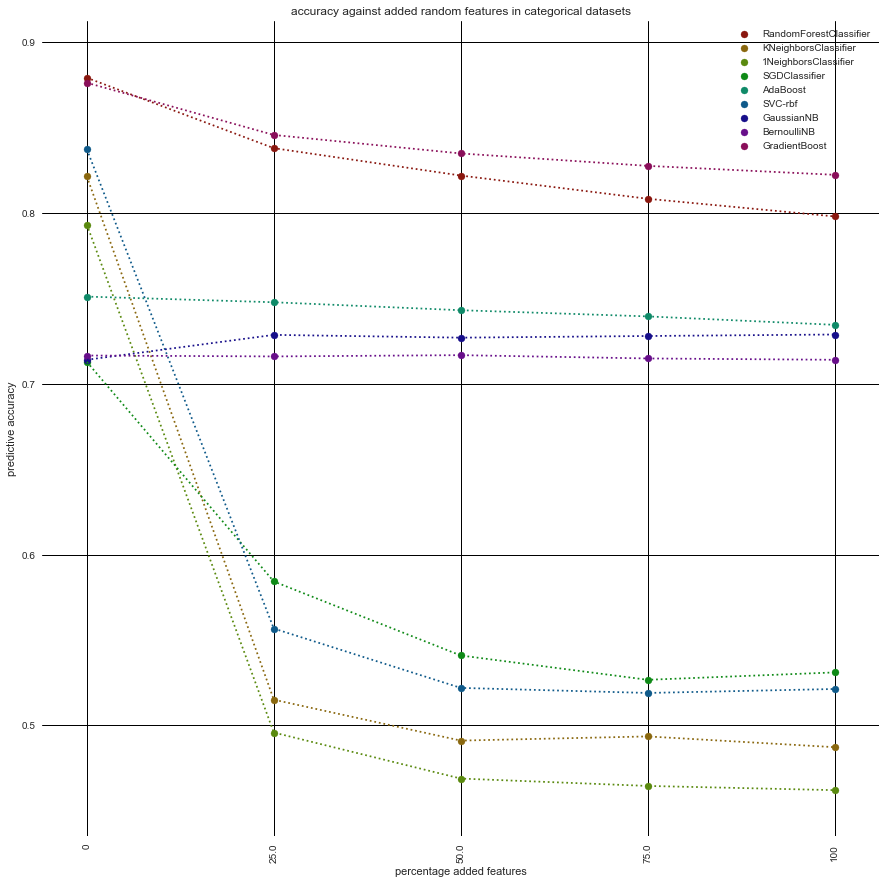
\includegraphics[
	width=0.65\textwidth
	]{images/RedudantFeature/predAddCatRand.png}
	\caption{Adding increasingly more random features(k = 100) to categorical datasets}
	\label{fig:predCatRand}
\end{subfigure}
	
	\caption{Predictive accuracy of categorical datasets injected with irrelevant or redundant features}
	\label{fig:predAddCat}
\end{figure}

\begin{figure}[H]
	\centering	
	\begin{subfigure}[b]{0.45\textwidth}
		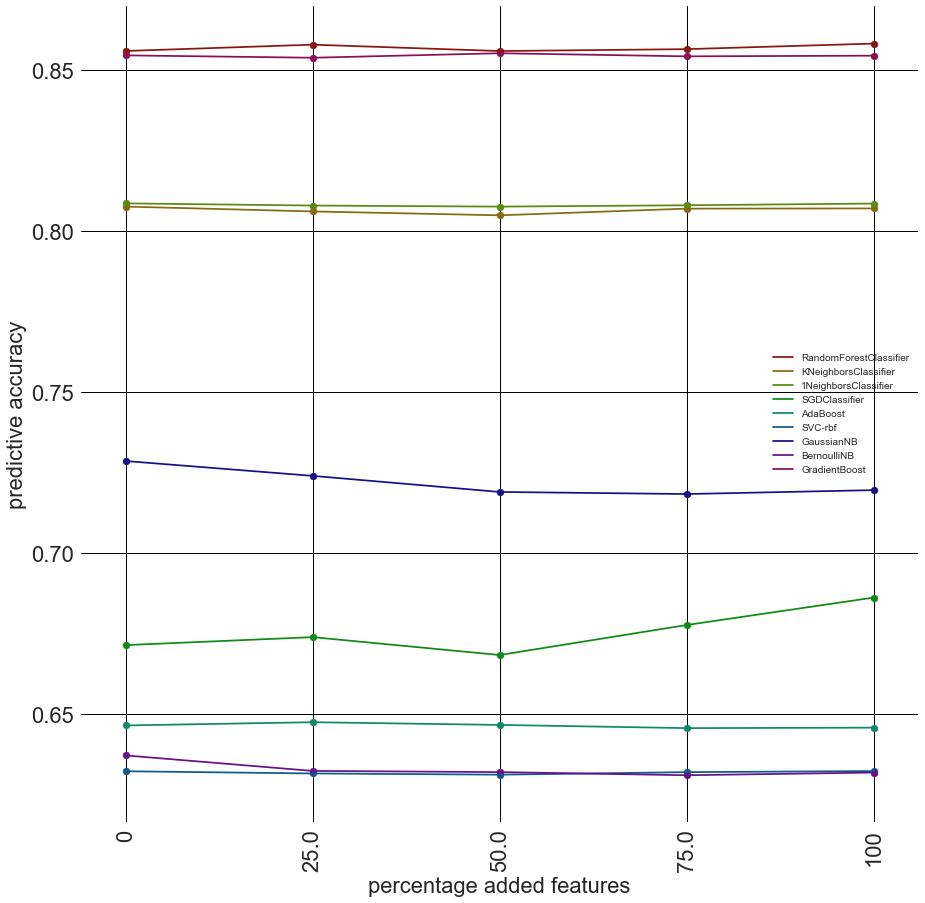
\includegraphics[
		width=0.65\textwidth
		]{images/RedudantFeature/predAddNumDup.png}
		\caption{Adding increasingly more duplicate features to numerical datasets}
		\label{fig:predNumDup}
	\end{subfigure}
	\begin{subfigure}[b]{0.45\textwidth}
		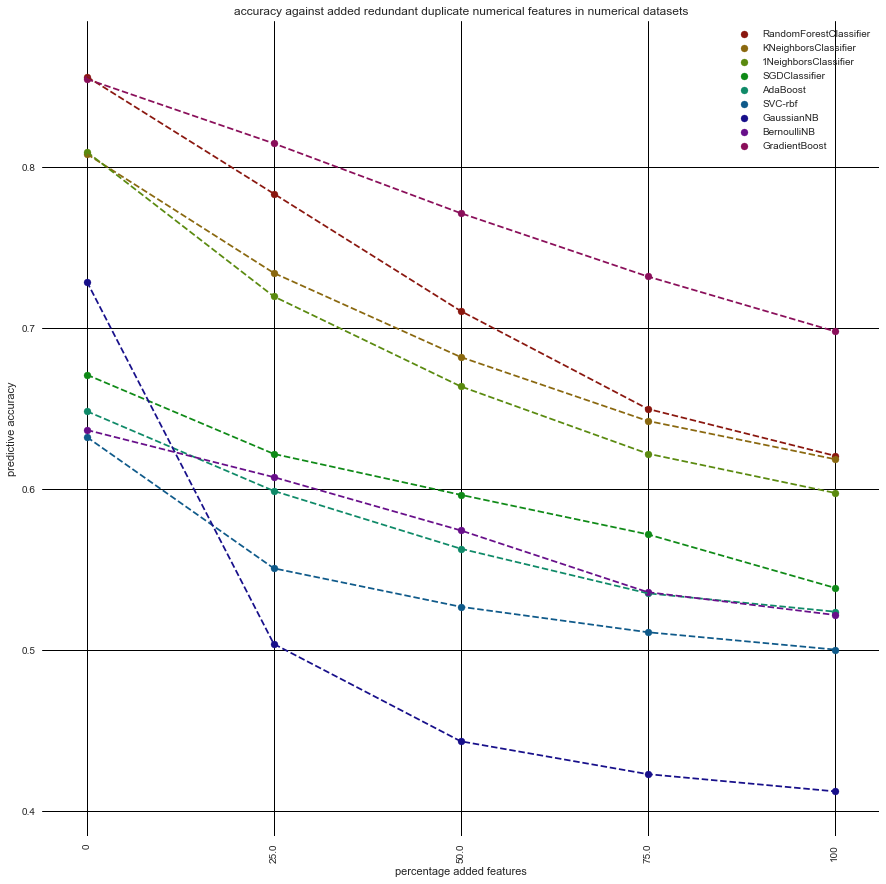
\includegraphics[
		width=0.65\textwidth
		]{images/RedudantFeature/predAddNumReDup.png}
		\caption{Adding increasingly more redundant duplicate features to numerical datasets}
		\label{fig:predNumReDup}
	\end{subfigure}
	\begin{subfigure}[b]{0.45\textwidth}
		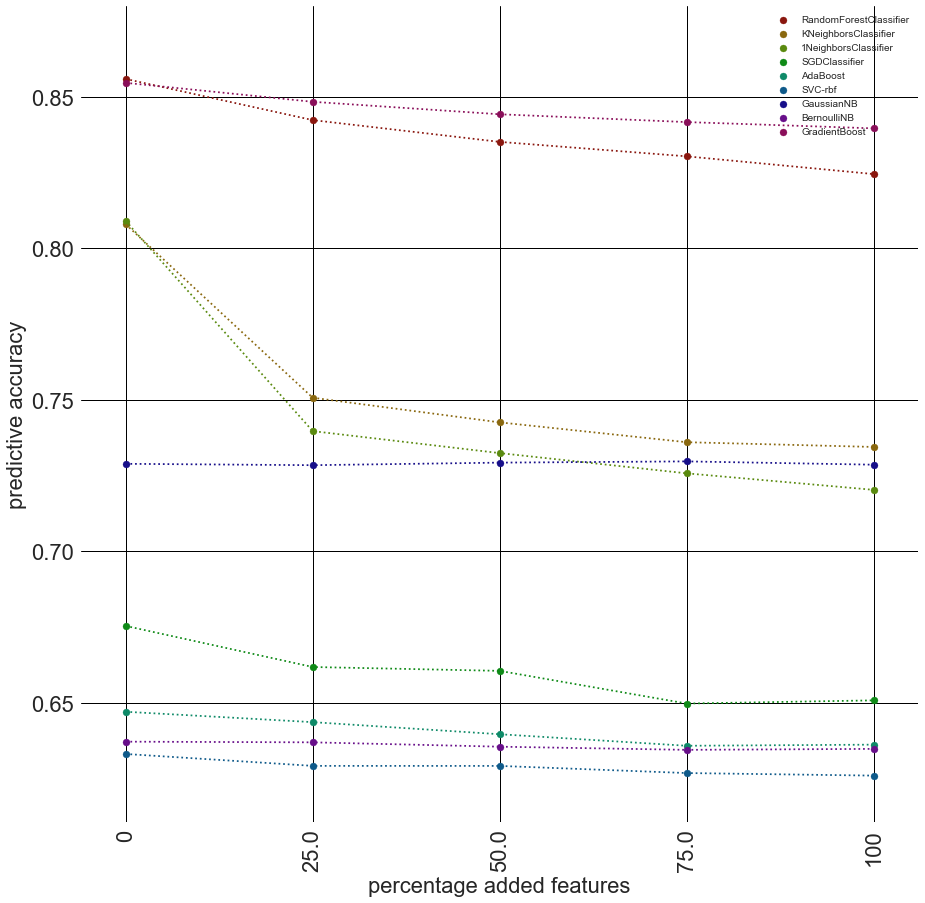
\includegraphics[
		width=0.65\textwidth
		]{images/RedudantFeature/predAddNumRand.png}
		\caption{Adding increasingly more random features to numerical datasets}
		\label{fig:predNumRand}
	\end{subfigure}
	
	\caption{Predictive accuracy of numerical datasets injected with irrelevant or redundant features}
	\label{fig:predAddNum}
\end{figure}




%TODO on hold asof 14/5 fault
\textbf{RandomForestClassifier} RandomForestClassifier is robust against default duplicate features with even gaining slightly better accuracy in both numerical and categorical datasets. The decrease in accuracy with adding redundant duplicate features is one of the hardest. As seen in chapter \ref{chapter312} RandomForestClassifier gives these added duplicate features less than its share of the dataset importance. The redundant duplciate feature have slightly more importance than the random numerical features and the result is far more decrease of accuracy for the redundant duplicate features. RandomForestClassifier is a ensemble method and therefor the performance does not drop dramatically on some redundant features but with a larger share the impact becomes more devisating.\\

\textbf{KNeighborsClassifier} The kNN classifier the robustness against duplciate feature is good for the default setting but for the 1NN there is more variance of performance for the categorical datasets. Adding the redundant features the kNN classifier is not so robust and the accuracy drops quickly. Against the random features the most impact can be seen when introducing the features. Upon introducting of the random categorical features the accuracy drops hard 30 $\%$ accuracy. For the numerical random features this is less but in comparison it is one of the largest drops in accuracy. THis is due the numbers associated with these random features. For the categorical features with k=100 the absolute difference between features become larger than with the default classes which are incremental categories. With a class feature value in the training set of 10 and a similair class with feature value 90 the absolute difference is large between features. Without preprocessing the kNN has no robustness against these irrelevant features. \\

\textbf{SGDClassifier} SGDClassifier is robust against duplicates with the random nature of the classifier. With added duplicates with numerical datasets the classifiers fluctuates a lot. With a doubled feature size the accuracy goes up a few percentages in accuracy. For categorical datasets the performance is less positive. Mostly for adding random categorical features the accuracy drops harshly. This is mostly because the SGDClassifier cannot handle categorical data nicely without preprocessing. The increase in number of classes and so more value variation makes is harder to use those features. The robustness for numerical datasets is stronger with average robustness for redundant duplicate features.  \\

\textbf{AdaBoost} The accuracy is hardly influence by duplicating features only for categorical datasets there is some slight variation between datasets. The robustness against redundant features is one of the greatest with subpar starting performance the drop in accuracy is fairly low. With similair reasons as RandomForestClassifier does the AdaBoost also give priority to the redundant duplicate features. For the random features AdaBoost is a robust classifier, with the focus on outliers AdaBoost can discredit these features as limiting the impact on the predictive accuracy. \\

\textbf{SVC-rbf} The robustness of SVC-rbf against duplicate features is similair to most classifiers. The lack of robustness against categorical datasts is mostly with the impact of these features. SVC-rbf builds on all features the decision surface and with these features being irrelevant the SVC has a harder time to correctly classify. Similair behaviour can be seen with the introduction of categorical random features. There are not misleading like redundant duplicate features but with the variation of 100 classes the SVC will fail to make a good decision surface without tuning of the C parameter to simplify the decision surface. There is more robustness for SVC with numerical random features. Handling of numerical redundant duplciate features is also not the strong suit of SVC but with a low accuracy the SVC is already underfitted on the data.  \\

\textbf{GaussianNB} GaussianNB is one of the only once to lose some accuracy with duplicate categorical features. With the added features the likelihood function has a decreased performance. The dependance on all the feature is also visible with the redundant feature addition for both categorical and numerical datasets the performance drops significantly with the introduction. The classifier depends on all features to fall in the distribution with a mean and variance and the added features fall outside these values and accuracy drops. For random categorical features the GaussianNB is even the most robust with an increase in accuracy with the introduction. For numerical the accuracy stays the same. This is by virtue of the random features having a clear structure of uniform randomness which the classifiers gives no importance to in classification accuracy.   \\

\textbf{BernoulliNB} Similair to GaussianNB does BernoulliNB lose accuracy with introduction of duplicate features. As a trait of a Naïve Bayes classifier all features are given some importance and these duplicate feature have equal perfomance as the original features. As this is mostly categorical datasets  the binarization of these feature decreases the accuracy. The redudant duplicate feature addition to the dataset decreases the accuracy only slightly as seen with the introduction of duplicates the accuracy can decrease with more irrelevant features. The decrease of accuracy of the BernoulliNB is the lowest which indicates that the classifier has hardly classified correctly because of underfitting. The result is that the accuracy drops only because it depends on all features useful for prediction calculated during fitting. The addition of random feature has a similair effect as on GaussianNB namely no effect. \\

\textbf{GradientBoostingClassifier} The effect of duplicate features has a similair story to both AdaBoost and RandomForestClassifier in other words no effect. The decision trees handle the duplicate features as a bit less important than the original dataset(figure {fig:FIGBC}). This explains a less decrease in accuracy compared to the RandomForestClassifier, the classifier is less fitted to those added features and so more robust. For the random features the same is true, as it shows better performance over the RandomForestClassifier. \\

\begin{table}[h]
	\centering
	\csvautotabular{flucRedudantFeatures.csv}
	\caption{all changes in predictive accuracy in adding both kind of features(results from figures \ref{fig:predAddNum} and \ref{fig:predAddCat})}\label{table:fluc}
\end{table}




\subsubsection{Combined feature manipulation}
\begin{figure}[h] 
	\centering
	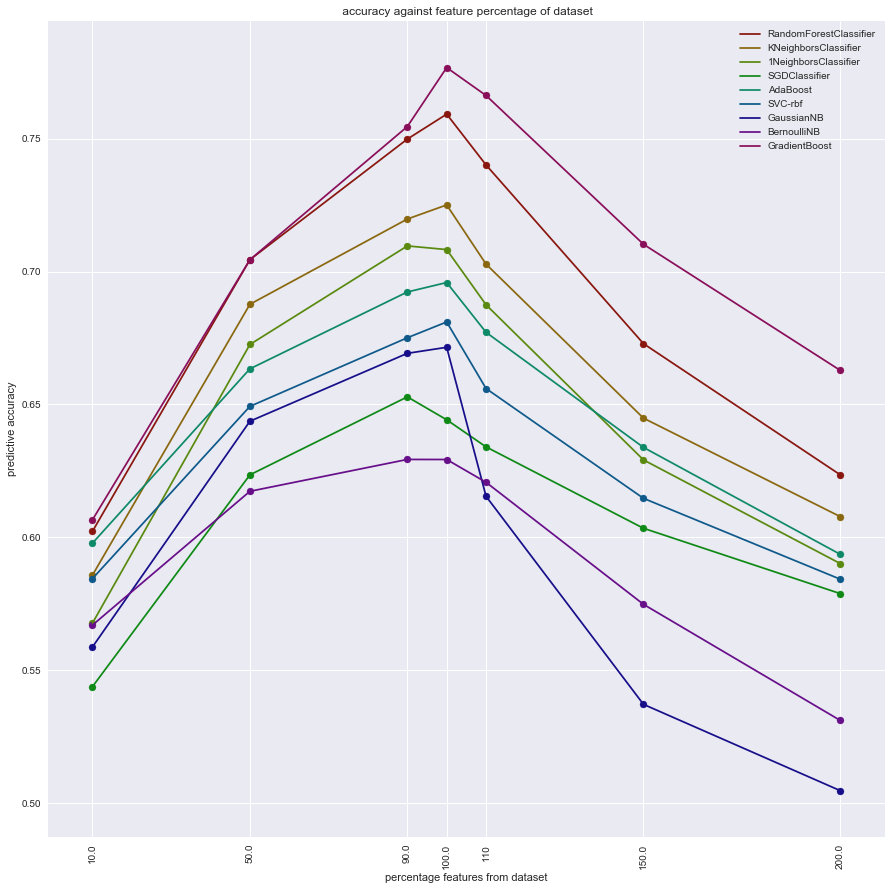
\includegraphics[
	width=0.65\textwidth
	]{images/RedudantFeature/predFeatureComplete.png}
	\caption{predictive accuracy for datasets with added or removed redundant features}
	\label{fig:preddFeatComp}
\end{figure}



\textbf{RandomForestClassifier}    \\

\textbf{KNeighborsClassifier} \\

\textbf{SGDClassifier} \\

\textbf{AdaBoost} \\

\textbf{SVC-rbf} \\

\textbf{GaussianNB} \\

\textbf{BernoulliNB} \\

\textbf{GradientBoostingClassifier} \\

\subsection{Noisy data}
Datasets in these experiments get increasingly more random by injecting the features with noise. In figures \ref{fig:predCatFeat}, \ref{fig:predNonCatFeat} and \ref{fig:predNonCatFeatPre} the accuracy against the noise are displayed. The noise consists of either flipping categories for categorical data or adding a random amount of standard deviation.
\begin{figure}[h] 
	\centering
	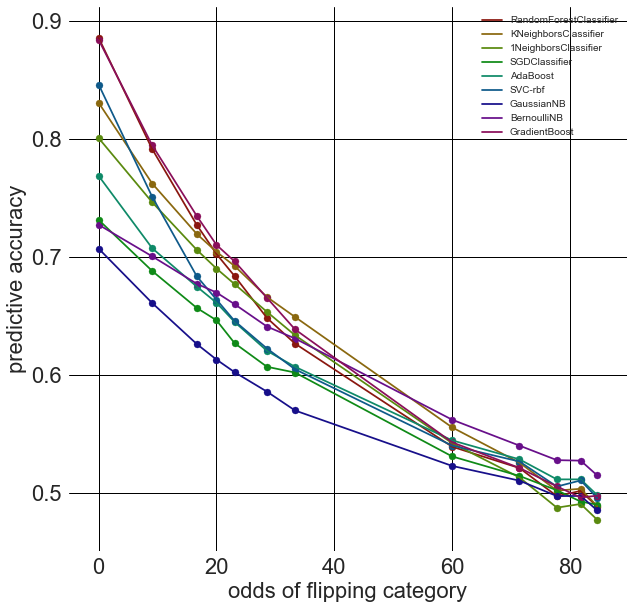
\includegraphics[
	width=0.65\textwidth
	]{images/NoisyFeatures/predCatFeat.png}
	\caption{flipping categories for categorical features}
	\label{fig:predCatFeat}
\end{figure}

\begin{figure}[h] 
	\centering
	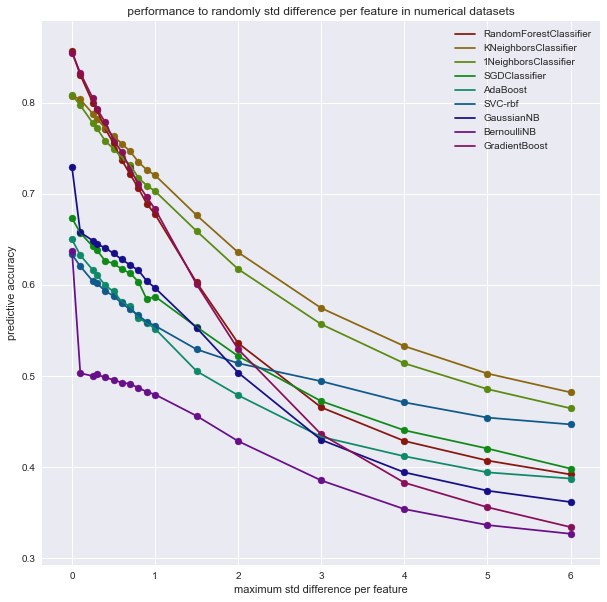
\includegraphics[
	width=0.65\textwidth
	]{images/NoisyFeatures/predNonCatFeat.png}
	\caption{adding or removing uniformly random std to numerical features}
	\label{fig:predNonCatFeat}
\end{figure}

\begin{figure}[h] 
	\centering
	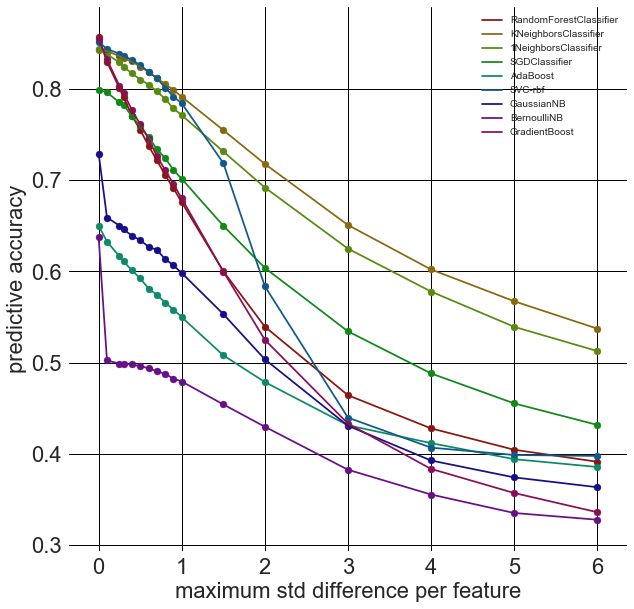
\includegraphics[
	width=0.65\textwidth
	]{images/NoisyFeatures/predNonCatFeatPre.png}
	\caption{adding or removing uniformly random std to numerical features and preprocessing for some classifiers.}
	\label{fig:predNonCatFeatPre}
\end{figure}

\textbf{RandomForestClassifier}: The accuracy of RandomForestClassifier is one of the best without optimization or cleaning the data. The decline in predictive accuracy is however far greater. This is because of the nature of a decision tree. The decision tree has numerical boundaries or categorical boundaries made on the original data set  to set apart the target classes. By adding the noise or flipping the categories these boundaries are blurred and the RandomForestClassifier has a higher chance to choose a different class, if in the original case it was straightforward. This makes the RandomForestClassifier not that robust against noisy data.  \\

\textbf{KNeighborsClassifier}: KNeighborsClassifier has a decent initial predictive accuracy and it is only slightly increased by the preprocessing. The downward trend of the influence of the noise is one of the least decending. The default 5 neighbors or 1 neighbor also has only a slight influence on accuracy. For the numerical datasets the initial accuracy on the clean dataset is equal and only after the added noise a clear difference is noticable which does not expand that much after 1 std.\\

\textbf{SGDClassifier}: SGDClassifier is not performing that well initially on either categorical or numerical datasets. The average accuracy on a clean dataset is one of the lowest of the 8 classifers. In Robustness the SGDClassifier scores better. With the clean dataset the decline is only below KNeighborsClassifier and SVC. With the preprocessing however it beats the SVC in robustness and has a greatly improved initial accuracy. \\

\textbf{AdaBoost}: AdaBoost does not perform that well on the datasets without preprocessing. The classifier optimizes on edge cases and without the noisy instances in the training set it has a hard time optimizing on things it has not seen yet. The decline in accuracy is in this case not that bad and on par with SGDClassifier. Considering that AdaBoost is not optimized and that the datasets are not all particularlly relevant for AdaBoost the performance is too be expected.\\

\textbf{SVC-rbf} SVC-rbf has great predictive accuracy on the categorical dataset but not so much with the numerical dataset. The robustness of SVC-rbf with the numerical dataset is pretty strong as it ends up as one of the best classifiers. This does not translate well with more cleaned data. With the preprocessing steps SVC-rbf has a high predictive accuracy but the decline is far greater. This can be attributed to a sort of overfitting on the initial clean data as the difference in decline is easily noticable between the two results. \\

\textbf{GaussianNB}: GaussianNB has the worst performance on the categorical datasets and a decent performance on the numerical datasets. The robustness is however pretty bad as there is a large initial drop when adding the noise for the numerical datasets. The decline there after is also very high which indicate a lack of robustness. This is largely due to the nature of the GaussianNB. It assumes a normal distribution with a mean and variance but a slight shift in the numbers changes a lot in the distribution of the datasets. In figure \ref{fig:predNoisyFeaturesGNB} the big drop can be noticed for a few datasets. A different trend can also be noticed of increased accuracy, those results are on unbalanced datasets. \\

\textbf{BernoulliNB} BernoulliNB has one of the worst predictive accuracy on both categorical and numerical datasets. The robustness is also really  bad on the numerical datasets. The accuracy has a large drop when a little bit of noise is added and only a decrease equal to the drop for the remainging added noise. For the categorical dataset a better robustness can be observed as it beats all others from the point that the datasets are 60$\%$ noise. This can be explained by the conversion the classifier does with the input. For categorical data this means that it depends on multiple features for its prediction. For numerical features it means that a slight change in data from the training to the prediction means the transformation does not work anymore. For some of the numerical datasets there are still only a few unique values and those are used like the categorical features. This explains the large drop for the numerical datasets.  \\

\textbf{GradientBoostingClassifier} GradientBoostingClassifier has one of the best predictive accuracy on both sorts of datasets. Performing near equal to RandomForestClassifier. In robustness it loses to RandomForestClassifier on numerical datasets and there is only a slight increase over the results on categorical datasets. The results of GradientBoostingClassifier copy those of RandomForestClassifier as they both use Decision trees for their ensembles. The lack of robustness on numerical datasets can be regarded as overfitting compared to the RandomForestClassifier. The GBC uses more time to fit the classifiers for an additive model rather than pure random voting.\\


\subsection{Bias variance}


\subsection{Ontology}
To present the results from all the experiments, this ranks the different classifiers on different aspects discussed.
These rankings can be compared to results from a review from 2007 of classification techniques \cite{RevClass}
The result will be a ranking of classifiers on different scales. The scales are:
\begin{itemize}
	\item training and prediction duration
	\item robustness to noise
	\item preprocessing needed
	\item initial prediction accuracy
\end{itemize} 


%\section{Discussion} \label{Chapter5}






\newpage
\section{Conclusion and discussion} \label{Chapter5}

\subsection{Discussion}

\subsubsection{Missed opportunities}
Within saving as many information obtainable from the algoritms a missed oppertunity is the probability prediction of all the test sets. 

Another missed collected data is the prediction of the training data. This data might not give a good indication of predictive accuracy but can give some valuable information of overfitting on the input data. This can be calculated as a difference in prediction results of the training and test set. For some classifiers this holds more than others. For example SGDClassifier which fits the inputted data as differentiable functions. Opposed to KNeighborsClassifier which will look up all the inputted data for neighbors which will match the training data for prediction. 

\subsubsection{Duration}
For the duration pictures some results are removed as they do not fall in line with the other results at all. By using the standard of the clean dataset which is calculated with each run we throw out any results changing more than 5$\%$ from another average.
The reason for these differences in duration is because of multiple used systems and other processes running during computation. 

\subsection{Resilience to noise}






\subsubsection{different approach}
Instead of measuring the influence of standard deviation, we tried to add standard values to all features, the problem with that is features have different deviation and some classifiers prefer a zero mean. The results were similair to injection std but more abrupt. Just changing(moving/word) all features for some datasets mend a drop in accuracy but the continuation of upping the number mend little to change accuracy further.




\subsection{replication of previous work}

\begin{figure}[H]
	\centering
	\begin{subfigure}[b]{0.45\textwidth}
		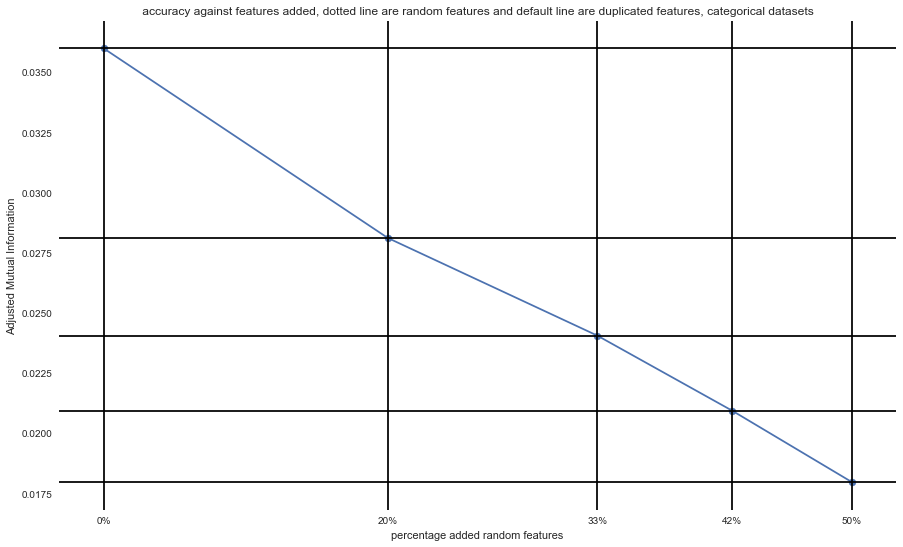
\includegraphics[width=\textwidth]{images/MutualInformationDecay.png}
		\caption{adjusted Mean Mutual Information for added random features.}
		\label{fig:AMMIdecay}
	\end{subfigure}
	\begin{subfigure}[b]{0.45\textwidth}
		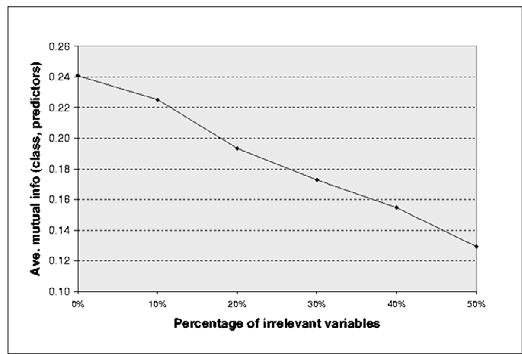
\includegraphics[width=\textwidth]{images/MutualInformationDecay-paper.png}
		\caption{average Mutual Information as a measure of relevance}
		\label{fig:AMMIpaper}
	\end{subfigure}
	\caption{Mutual information decline between previous work and this work}\label{fig:MMIs}
	\label{paper-thesis}
\end{figure}

In figure \ref{paper-thesis} the experiment setup of Hilario and the expriment setup of this thesis are shown\cite{Resil-1}. For Hilario it was to show that with the added random features the mutual information decreases an indicator that the added features could not improve the accuracy. In the experiment of this thesis the added features also show a decrease in mutual information but the mean mutual information scale is 10 times smaller. This indicates that the datasets used are less valueable in contrast to the ones used by Hilario. The change of x-scale compared to previous experiments is to able to compare it more to the work of Hilario. Comparing the results is harder as the versions of the classifiers have been changed over time.


%\subsection{New discoveries}




\subsection{Future work}
%\subsubsection{More computation}
Adding more experimental runs to this topic can further solidify the results, break the result or alter only slightly the results. As benchmark datasets have a hard time to be a universal standard for testing. The results of a golden standard benchmark may also limit results because of the no free lunch theorem

A source of attention can be the use of that only datasets available on openml are used. Openml has a certain community and the datasets available on Openml may not translate to other areas of interest. Another party to consider then is a platform like Kaggle which share a lot of datasets already but the commercial side to kaggle may be more of a counterpart to Openml. 

A partly solution for the previous mentioned problem of datasets is the splitting of datasets in certain categories. In this thesis there was a split for categorical and numerical features possible by the classification in Openml of all inputted features. Different splitting of dataset can be done in categories like sparse/dense or cleaned and uncleaned. Further distinguishing in categorical and numerical featueres the different values of discrete, continous or ordinal values. Each can need different preproccessing steps for different classifiers. 






\section{References}
\begingroup
\begin{thebibliography}{9}
\bibitem{Data-science} The Popularity of Data Science Software, Robert A. Muenchen, r4stats.com, (2017)
\bibitem{python-pop} Most Popular Programming Languages For Machine Learning And Data Science,Adarsh Verma, fossbytes.com, (2016)
\bibitem{ML-trends} 
Machine learning: Trends, perspectives, and prospects, M. I. Jordan, T. M. Mitchell, Science Volume 349 issue 6245 pages 255-260, (2015)
\bibitem{Big-data} Storage predictions: Will the explosion of data in 2017 be repeated in 2018?, Nick Ismail, www.information-age.com/, (2017)
\bibitem{Joaquin-phd} Understanding Machine Learning Performance with experiment databases, Joaquin Vanschoren, KU Leuven, (2010)
\bibitem{Resil-1} Quantifying the resilience of inductive classification algorithms, M. Hilario, A. Kalousis, 
Proceedings of the 4th European Conference on Principles of data mining and knowledge discovery, pages 106-115, (2000)
\bibitem{Sam-var}Updating Formulae and a Pairwise Algorithm for Computing Sample Variances Tony F. Chan* Gene H. Golub’* Randall J. LeVeque, Stanford CS tech report STAN-CS-79-773(1979)
\bibitem{SVM}LIBSVM: A library for support vector machines, Chang, Chih-Chung, Lin, Chih-Jen, ACM Transactions on Intelligent Systems and Technology (2011)
\bibitem{Multi-pair-coup} Probability estimates for multi-class classification by pairwise coupling, Wu, Lin, Weng, Journal of Machine Learning Research 5 (2004)
\bibitem{SVN} Support-Vector networks, Cortes, Corinna, Vapnik, Vladimir, Machine Learning Volume 20 issue 3 (1995)
\bibitem{Bayes} Idiot’s Bayes—Not So Stupid After All?, David J. Hand, Keming Yu, International Statistical Review Volume 69 Number 3(2001)
\bibitem{NB-text} A Comparison of event models for naïve Bayes text classification, Andrew McCallum, Kamal Nigam, AAAI-98 workshops on learning for text categorization (1998)
\bibitem{KNN-k} Investigating the performance of Naive-bayes classifiers and k-nearest neighbor classifiers, M. J. Islam, Q. M. J. Wu, M. Ahmadi and M. A. Sid-Ahmed, International conference on convergence information technology(ICCIT) Gyeongju pages 1541-1546,(2007)
\bibitem{RDF} Random Decision Forests, Tin Kam Ho, Proceedings of the 3rd Iternational Conference on Document analysis and recognition (1995)
\bibitem{AdaBoost} A short introduction to Boosting, Yoav Freund, Robert E. Shapire, Journal of Japanse Society for artificial Intelligence 14(5):771-780 (1999)
\bibitem{MadaB} Multi-class AdaBoost, J. Zhu, S. Rosset, H. Zou, T. Hastie, Statistics and its Interface volume 2, pages 349-360 (2009)
\bibitem{SGDClass} Solving Large Scale Linear Prediction problems using stochastic gradient descent algorithms, T. Zhang, ICML Proceedings of the 21 International conference on machine learning (2004)
\bibitem{GradientBoost} Stochastic Gradient Boosting, J. H. Friedman,  Computational Statistics \& Data analysis – Nonlinear methods and data mining volume 38 issue 4 pages 367-378,(2002)
\bibitem{Greedy-GBC} Greedy function approximation: A gradient boosting machine, J. H. Friedman, The annals of statistics volume 29 issue 5, pages 1189-1232,(2001)
Previous bias-variance research has shown a trend of larger dataset increasing the bias component but still fluctuating with  less than 10000 instances.
\bibitem{Bias-var} Experiment databases, J. Vanschoren, H. Blockeel, B. Pfahringer, G. Holmes, Machine Learning Volume 82 issue 2 pages 127-158, (2012)
\bibitem{BiasCalc} Bias plus variance decomposition for zero-one loss functions,R. Kohavi, D. Wolpert, Proceedings of the international conference on machine learning pages 275-283,(1996)
\bibitem{RevClass} Supervised Machine Learning: A review of classification techniques, S.B. Kotsiantis, Informatica 31, (2007)
\bibitem{ranking} Pairwise meta-rules for better meta-learning-based algorithm ranking, Quan Sun, Bernhard Pfahringer, Machine Learning Volume 93 Issue 1 pages 141-161,(2013)
\bibitem{Sklearn-Bench} Scikit-learn: Machine Learning in python, F. Pedregosa, G. Varoquaux, A. Gramfort, V. Michel, B. Thirion et al. Journal of Machine Learning Research 12, (2011)
\bibitem{No-Free-Lunch} No free lunch theorems for optimization, D.H. Wolpert, W.G. Macready, IEEE Transactions on Evolutionary Computation Volume 1 Issue 1, (1997)
\bibitem{KNN-Sym} A Weighted Nearest Neighbor Algorithm for Learning with symbolic features, S. Cost, S. Salzberg, Machine Learning Volume 10, number 1 pages 57-78, (1993)
\bibitem{SVM-sym} A practical guide to support vector classification, Chih-wei Hsu, Chich-Chung Chang, Chich-Jen Lin, 101. 1396-1400, (2003)
\bibitem{Cross} A study of cross-validation and bootstrap for accuracy estimation and model selection, R. Kohavi, (1995)
\bibitem{KNN} Nearest neighbor pattern classification, T. Coverm P. Hart, IEEE Transaction on Information Theory 13:21-27,(1967)




 
     
\end{thebibliography}
\endgroup

\section{Appendix}
\subsection{datasets}
\subsubsection{datasets per figure}
openml dataset identifiers per figure \\
figure \ref{fig:predFlat} - 10,12,18 \\
figure \ref{fig:FailDurMan} - 1038,1043,1049,1050,1176,12,1466,1468,1475,1476,1478,1479,1485,1487,1491,1492,1493,1494,14,1501,1504,1510,1515,16,22,28,300,40499,40,4134,44,4538,458 \\
figure \ref{fig:FeatManLog} - 22, 1176, 4134, 1063, 1067, 1068, 44, 53, 4538, 458 \\
figure \ref{fig:FeatCorImp} - 12, 1038, 14, 16, 1043, 22, 1176, 1049, 1050, 28, 1063, 1067, 1068, 300, 1466, 1467, 1468, 1475, 1476 \\
figure \ref{fig:FeatRemImp} - 1038, 1043, 22, 1176, 1049, 1050, 1063, 1067, 1068
figure \ref{fig:predAddNum} - 11, 12, 1038,14, 16, 18, 1043, 1046, 22,1176, 1049, 1050, 28,30, 32, 1570, 36, 37, 4134, 1063, 39, 40, 1067, 1068, 300, 41, 44, 1459, 40499 , 53, 1462, 1464, 54, 1466, 1467, 1468, 40509, 4538, 1475, 1476, 1478, 1479, 458,1485, 1487, 1489, 1491, 1492, 1493, 1494, 1497, 1501, 1504, 1510, 1515, 375\\ 
figure \ref{fig:predAddCat} - 20, 21, 26, 333, 334, 335, 40668, 4135, 4534, 469, 46, 50\\
\subsubsection{Distribution}
The number of features and instances for datasets
\begin{figure}[h] 
	\centering
	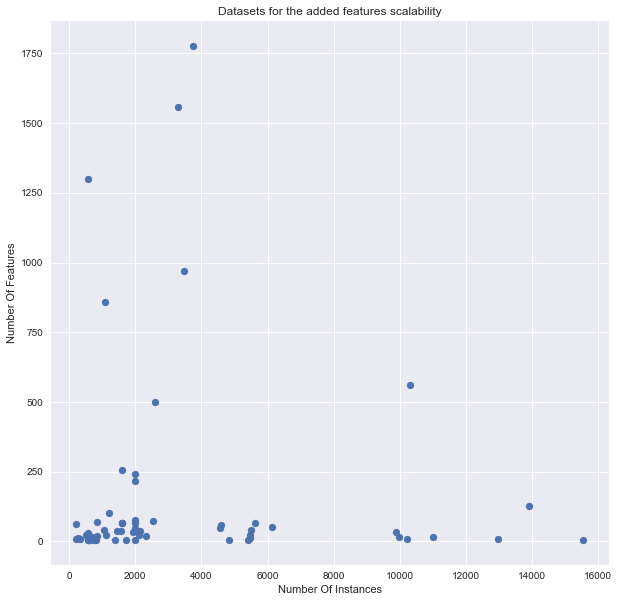
\includegraphics[
	width=0.65\textwidth
	]{images/appendix/ScalabilityAdd.png}
	\caption{Dataset metafeatures for figure \ref{fig:ScalableAdded}}
	\label{fig:distrAdd}
\end{figure}


\subsection{different approach}
\begin{figure}[h] 
	\centering
	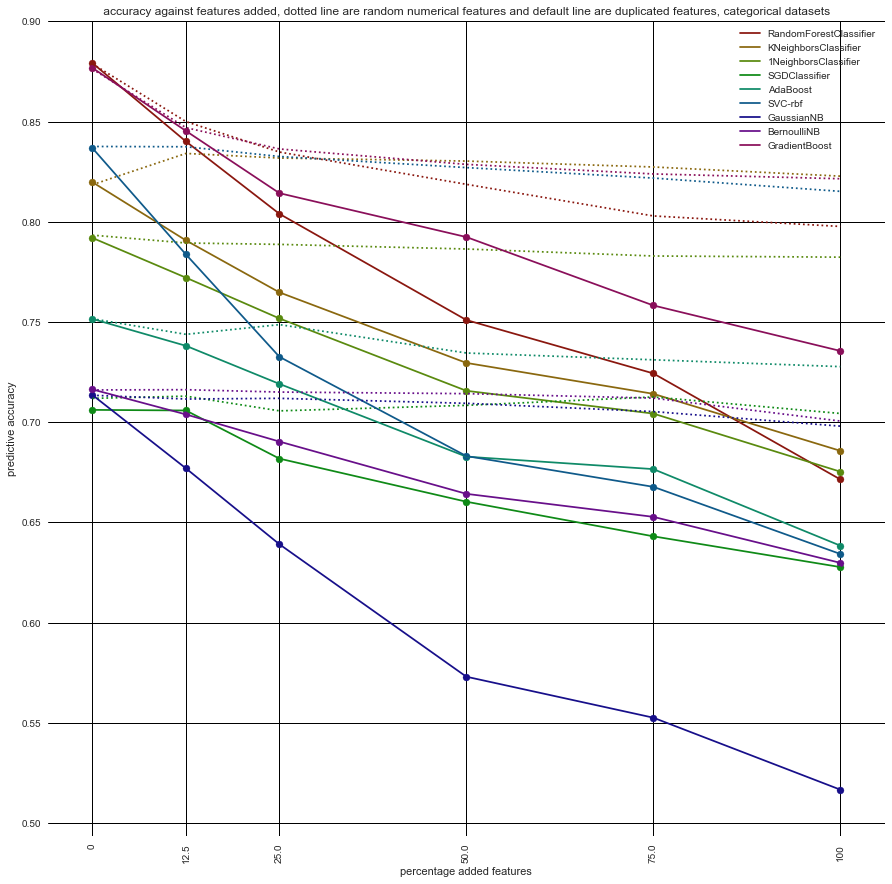
\includegraphics[
	width=0.65\textwidth
	]{images/appendix/predRedudantFeaturesCatNum.png}
	\caption{adding or removing uniformly random std to numerical features for GaussianNB.}
	\label{fig:predRedCatNum}
\end{figure}

\begin{figure}[h] 
	\centering
	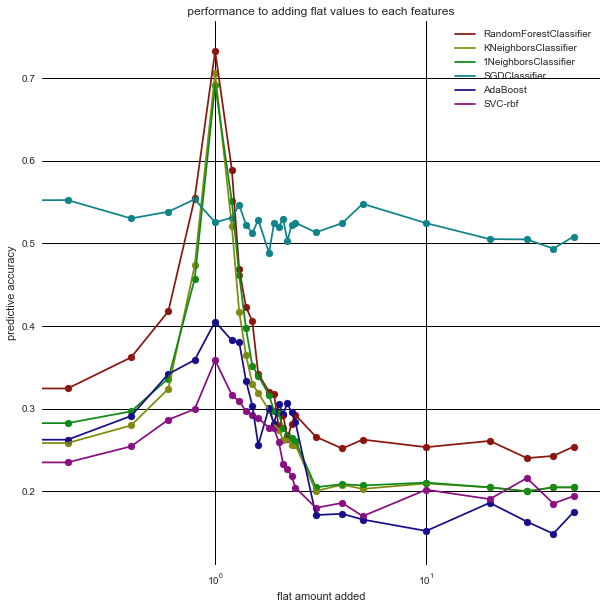
\includegraphics[
	width=0.65\textwidth
	]{images/appendix/predFlat.png}
	\caption{adding flat values to each feature}
	\label{fig:predFlat}
\end{figure}

\subsection{Duration variance}
In this section duration examples are shown which show behaviour that should not happen.
\begin{figure}[h] 
	\centering
	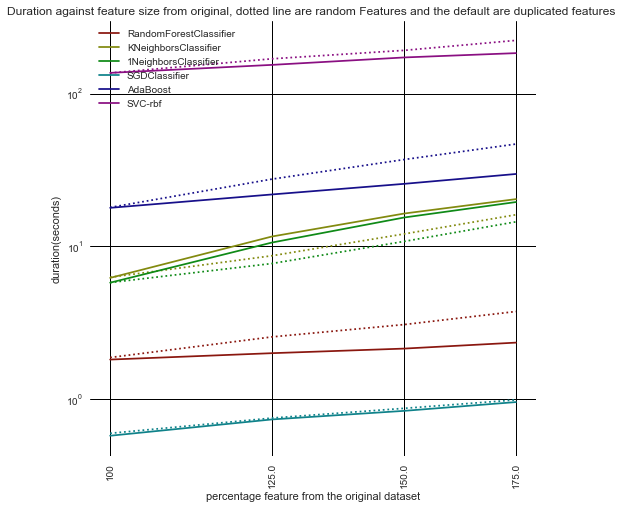
\includegraphics[
	width=0.65\textwidth
	]{images/appendix/DurAddOld.png}
	\caption{Duration of the oldest version of adding random features}
	\label{fig:durOld}
\end{figure}

\begin{figure}[h] 
	\centering
	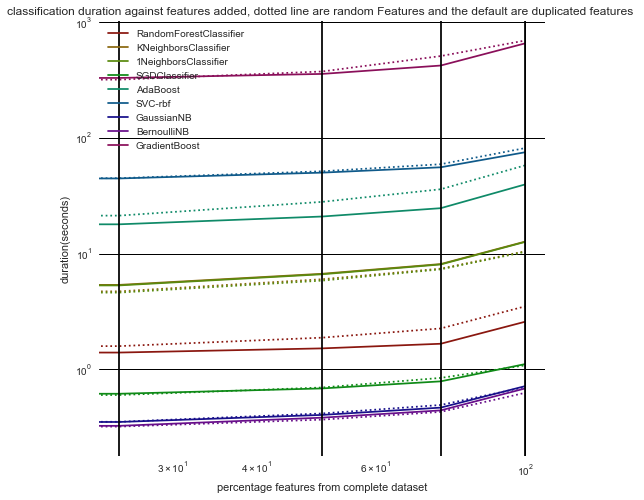
\includegraphics[
	width=0.65\textwidth
	]{images/appendix/FailDurAdd.png}
	\caption{Duration of the oldest version of adding random features}
	\label{fig:durNewer}
\end{figure}

\begin{figure}[h] 
	\centering
	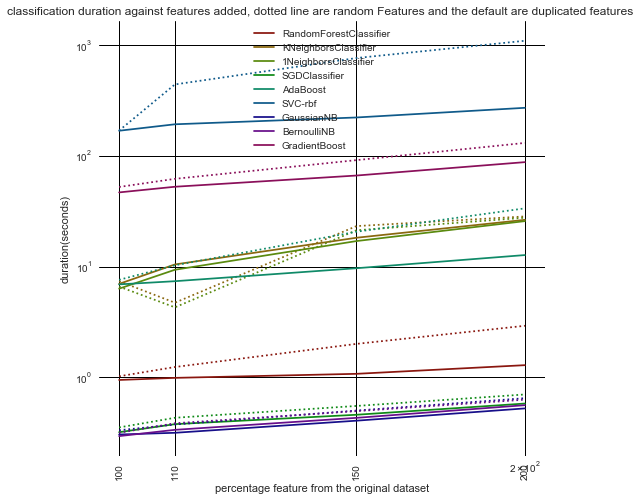
\includegraphics[
	width=0.65\textwidth
	]{images/appendix/FailDurAddNew.png}
	\caption{Duration of the newest version of adding random features}
	\label{fig:durNewest}
\end{figure}

\begin{figure}[h] 
	\centering
	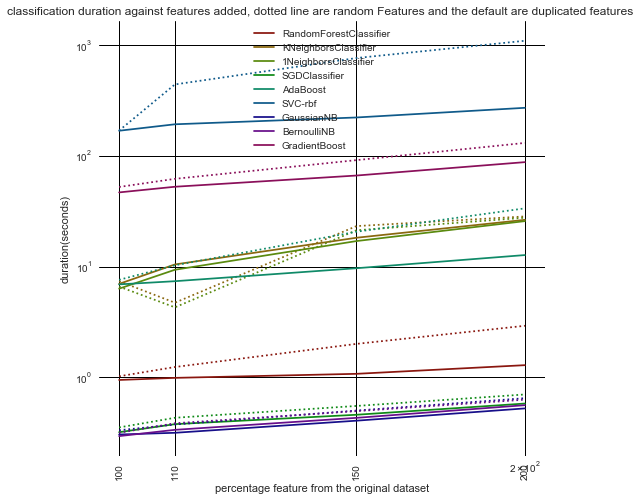
\includegraphics[
	width=0.65\textwidth
	]{images/appendix/FailDurAddNew.png}
	\caption{Duration of the newest version of adding random features}
	\label{fig:durNewest}
\end{figure}

\begin{figure}[h] 
	\centering
	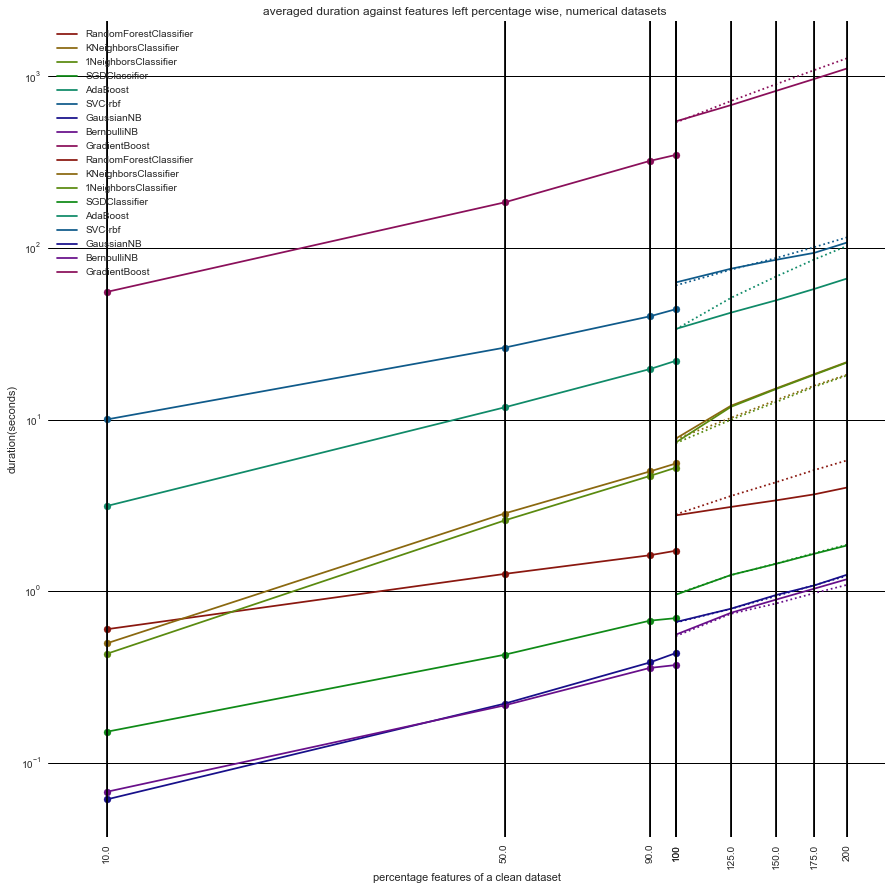
\includegraphics[
	width=0.65\textwidth
	]{images/appendix/FailDurMan.png}
	\caption{Duration of adding and removing features combined result}
	\label{fig:FailDurMan}
\end{figure}

\begin{figure}[h] 
	\centering
	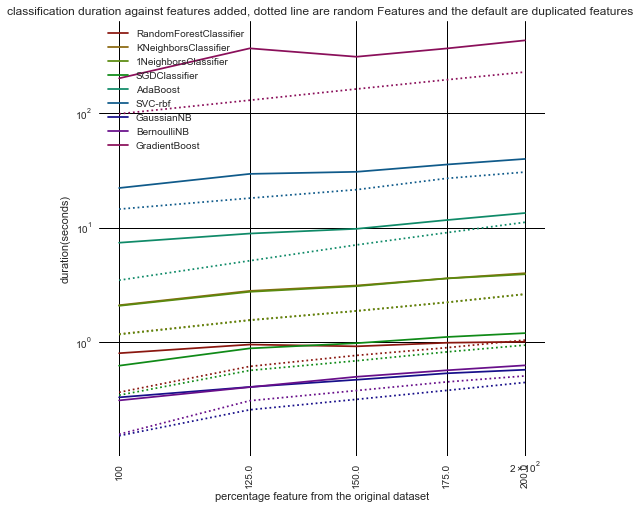
\includegraphics[
	width=0.65\textwidth
	]{images/appendix/FailFixedDup.png}
	\caption{Duration of duplicated features against random features with clear spikes in duration registering}
	\label{fig:failFixed}
\end{figure}



\newpage
\subsection{Results per dataset per classifier}
\begin{figure}[h] 
	\centering
	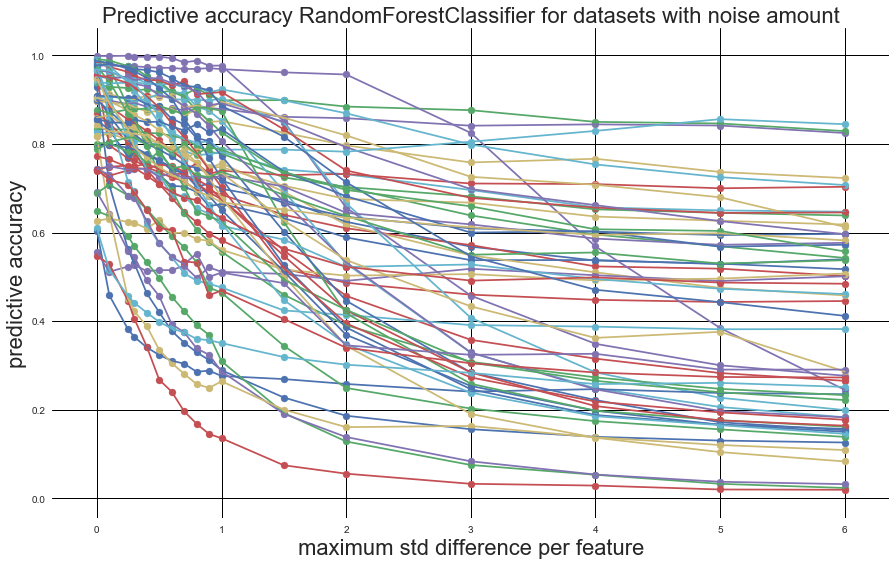
\includegraphics[
	width=0.65\textwidth
	]{images/appendix/PredNoisyFeaturesRF.png}
	\caption{adding or removing uniformly random std to numerical features for RandomForestClassifier.}
	\label{fig:predNoisyFeaturesRF}
\end{figure}
\begin{figure}[h] 
	\centering
	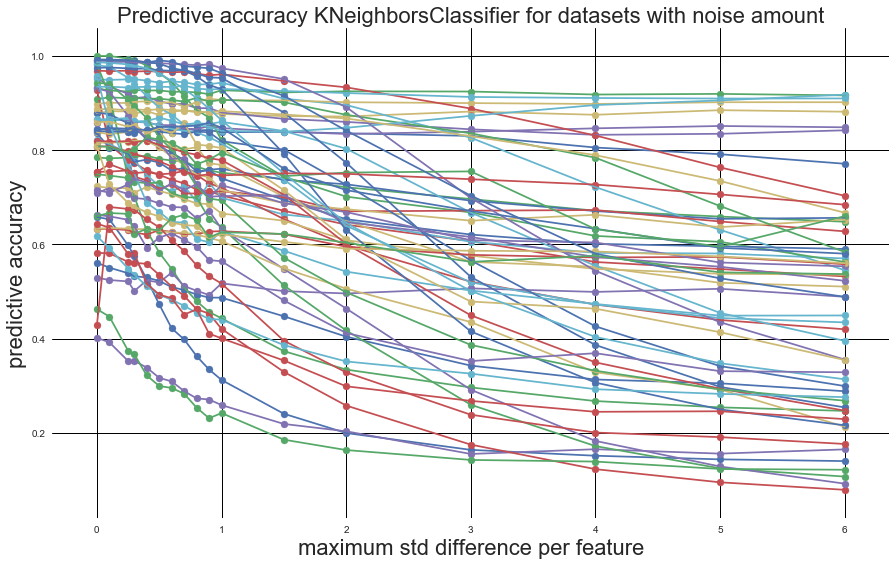
\includegraphics[
	width=0.65\textwidth
	]{images/appendix/PredNoisyFeaturesKNN.png}
	\caption{adding or removing uniformly random std to numerical features for KNeighborsClassifier.}
	\label{fig:predNoisyFeaturesKNN}
\end{figure}
\begin{figure}[h] 
	\centering
	\includegraphics[
	width=0.65\textwidth
	]{images/appendix/PredNoisyFeatures1NN.png}
	\caption{adding or removing uniformly random std to numerical features for 1NeighborClassifier.}
	\label{fig:predNoisyFeatures1NN}
\end{figure}
\begin{figure}[h] 
	\centering
	\includegraphics[
	width=0.65\textwidth
	]{images/appendix/PredNoisyFeaturesSGD.png}
	\caption{adding or removing uniformly random std to numerical features for SGDClassifier.}
	\label{fig:predNoisyFeaturesSGD}
\end{figure}
\begin{figure}[h] 
	\centering
	\includegraphics[
	width=0.65\textwidth
	]{images/appendix/PredNoisyFeaturesADA.png}
	\caption{adding or removing uniformly random std to numerical features for AdaBoost.}
	\label{fig:predNoisyFeaturesADA}
\end{figure}
\begin{figure}[h] 
	\centering
	\includegraphics[
	width=0.65\textwidth
	]{images/appendix/PredNoisyFeaturesSVC.png}
	\caption{adding or removing uniformly random std to numerical features for SVC-rbf.}
	\label{fig:predNoisyFeaturesSVC}
\end{figure}
\begin{figure}[h] 
	\centering
	\includegraphics[
	width=0.65\textwidth
	]{images/appendix/PredNoisyFeaturesGNB.png}
	\caption{adding or removing uniformly random std to numerical features for GaussianNB.}
	\label{fig:predNoisyFeaturesGNB}
\end{figure}
\begin{figure}[h] 
	\centering
	\includegraphics[
	width=0.65\textwidth
	]{images/appendix/PredNoisyFeaturesBNB.png}
	\caption{adding or removing uniformly random std to numerical features for BernoulliNB.}
	\label{fig:predNoisyFeaturesBNB}
\end{figure}
\begin{figure}[h] 
	\centering
	\includegraphics[
	width=0.65\textwidth
	]{images/appendix/PredNoisyFeaturesGBC.png}
	\caption{adding or removing uniformly random std to numerical features for GradientBoostingAlgorithm.}
	\label{fig:predNoisyFeaturesGBC}
\end{figure}
%insert tables

\end{document}